%%%%%%%%%%%%%%%%%%%%%%%%%%%%%%%%%%%%%%%%%%%%%%%%%%%%%%%%%%%%%%%%%%%%%%%%%%%%%%%%%%%
\section{Aim}
\label{sec:3aim}
%%%%%%%%%%%%%%%%%%%%%%%%%%%%%%%%%%%%%%%%%%%%%%%%%%%%%%%%%%%%%%%%%%%%%%%%%%%%%%%%%%%

Create an exposure model for \gls{pm25} on the London Underground

%%%%%%%%%%%%%%%%%%%%%%%%%%%%%%%%%%%%%%%%%%%%%%%%%%%%%%%%%%%%%%%%%%%%%%%%%%%%%%%%%%%
\section{Objectives}
\label{sec:3objectives}
%%%%%%%%%%%%%%%%%%%%%%%%%%%%%%%%%%%%%%%%%%%%%%%%%%%%%%%%%%%%%%%%%%%%%%%%%%%%%%%%%%%

\begin{itemize}
\item Measure \gls{pm25} across the London Underground network
\item Transcribe a time-location diary and link to pollutant data
\item Import other relevant data
\item Analyse data to characterise \gls{pm25} on the London Underground
\end{itemize}

%%%%%%%%%%%%%%%%%%%%%%%%%%%%%%
\section{Background}
\label{sec:3background}
%%%%%%%%%%%%%%%%%%%%%%%%%%%%%%

The London Underground (otherwise known as 'The Tube') has around 402 kilometres of track covering the Greater London Area, around which 52\% is overground and 48\% is underground (\cite{TransportforLondon2014a}). The network currently has annual passenger numbers of 1.305 billion, and is the main source of transport for the population of London. 

\begin{figure}[H]
\centering
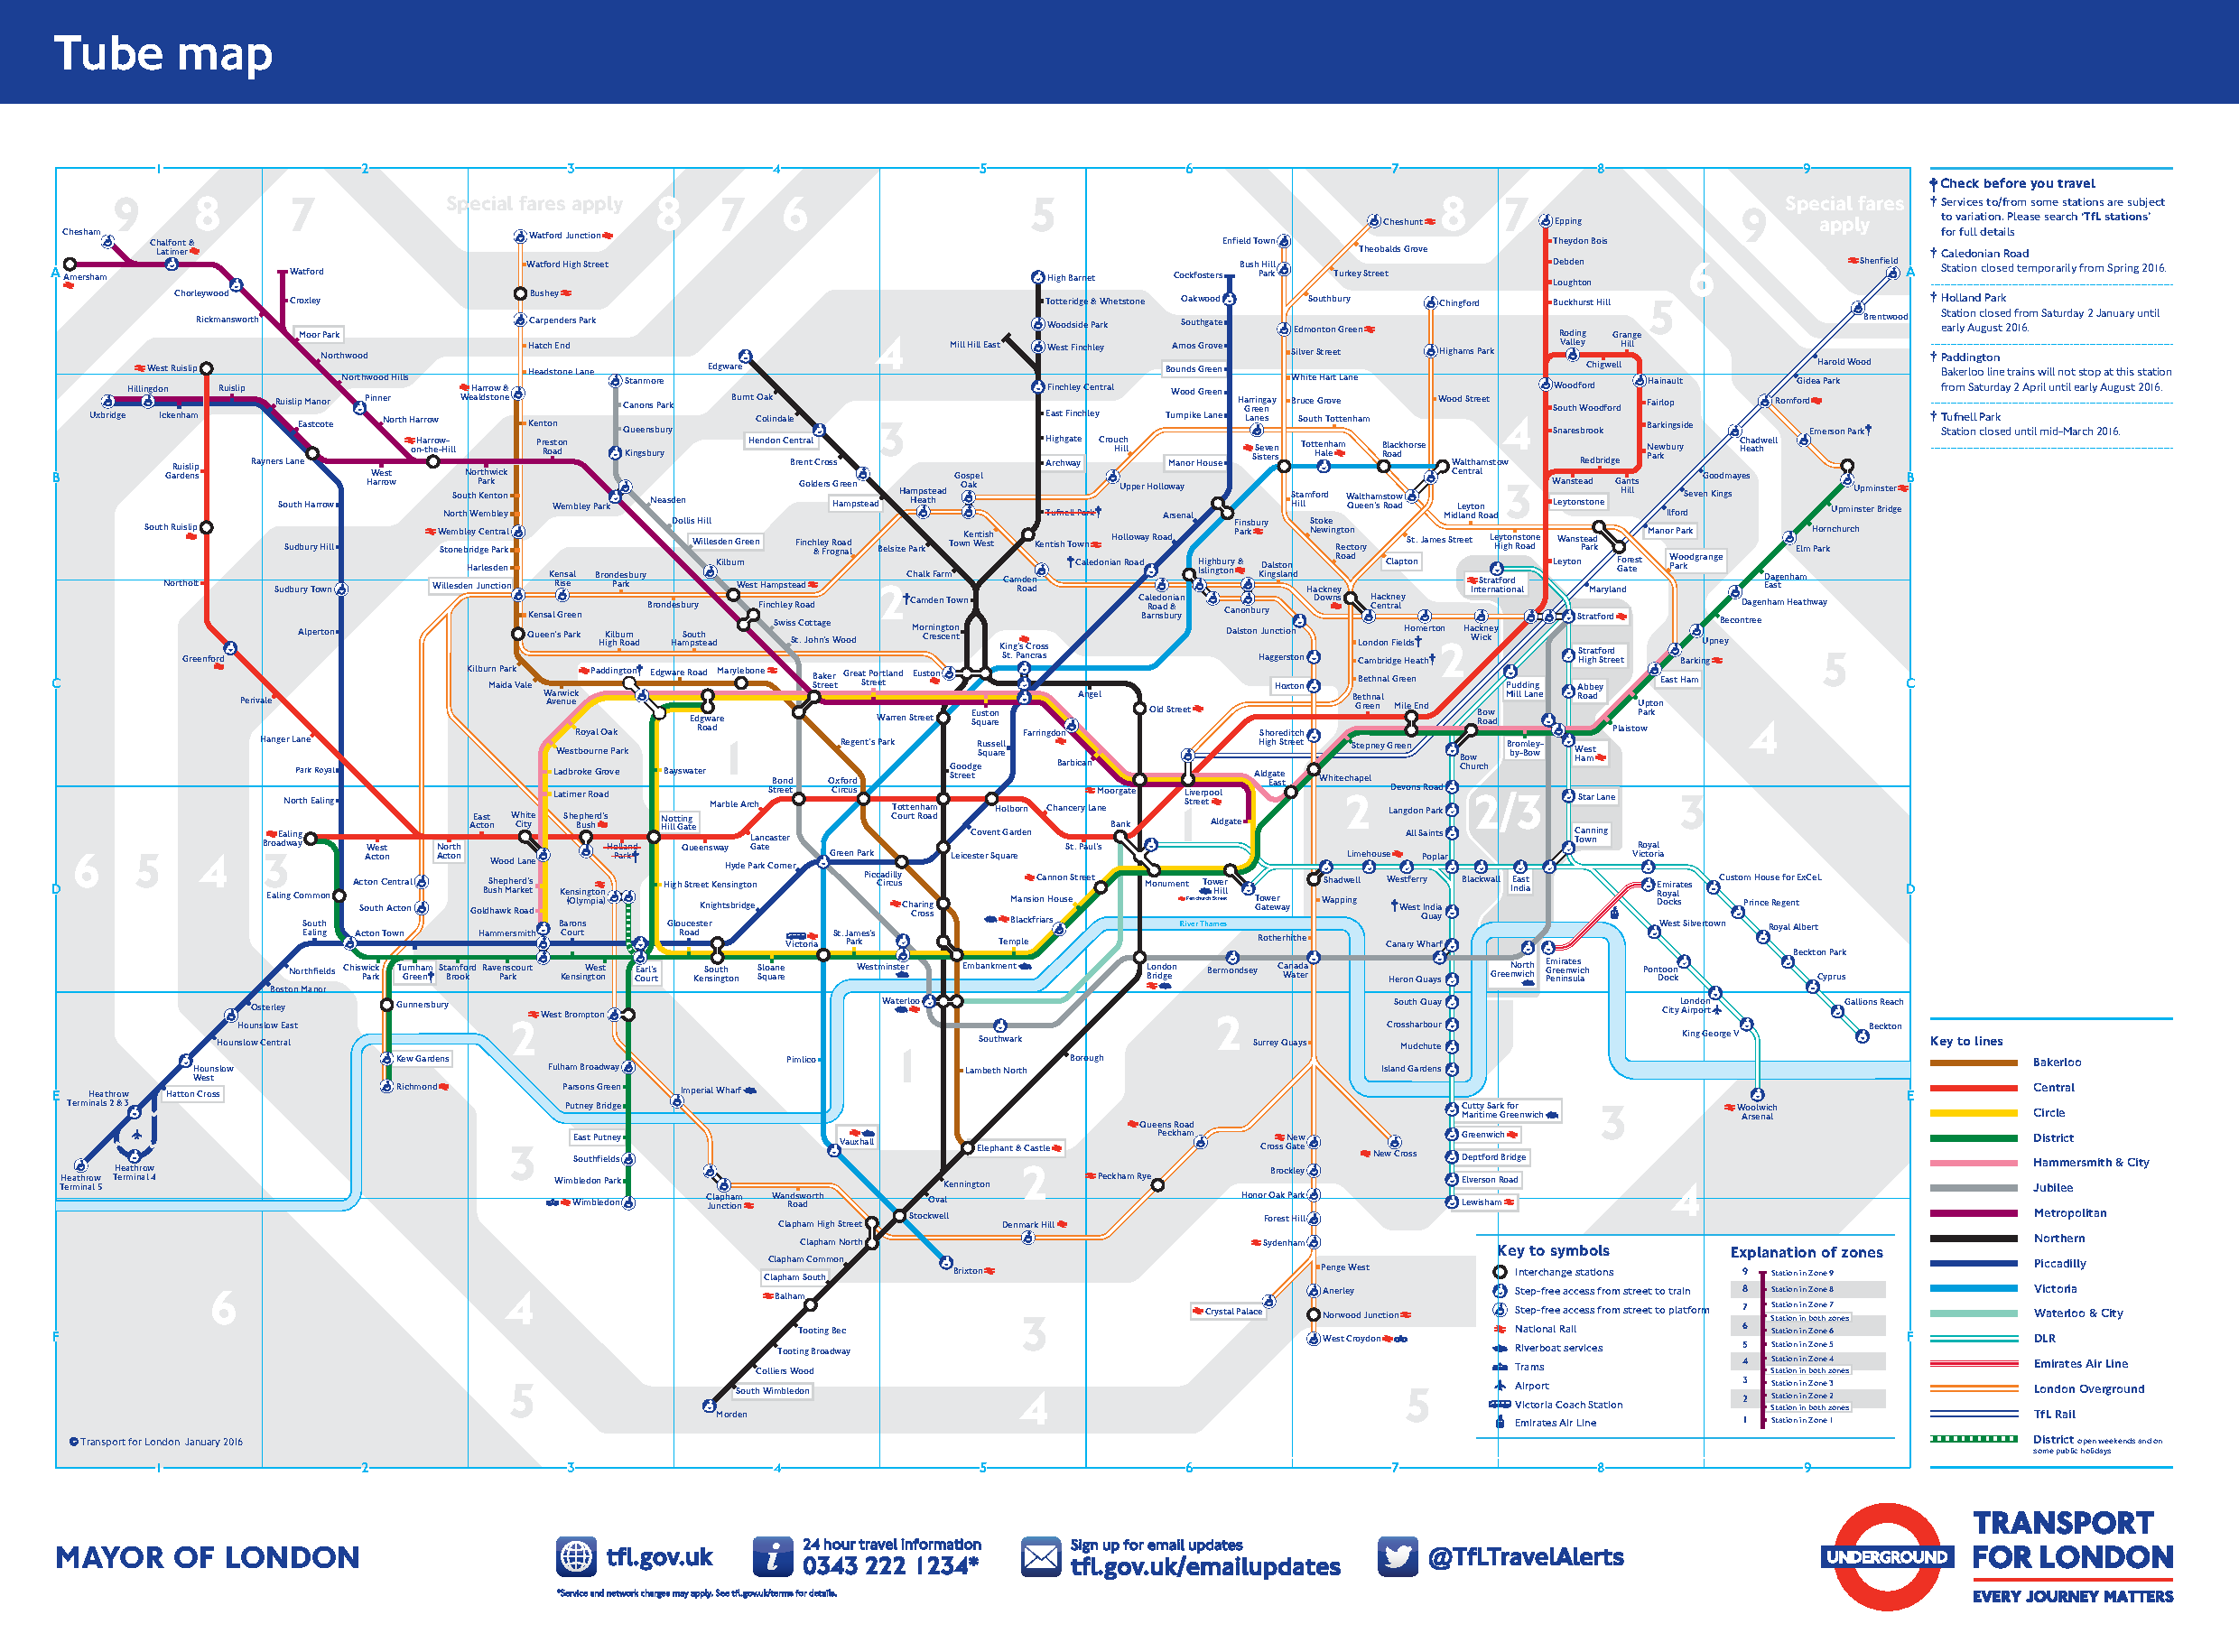
\includegraphics[scale=0.35]{tube_map}
\caption{A map of the London Underground}
\label{fig:tube_map}
\end{figure}

In the previous chapter concentrations of 94 $\mu \text{g m}^{-3}$ and 51 $\mu \text{g m}^{-3}$ for \gls{pm25} and \gls{no2} respectively were used as simple exposure estimates to represent exposure while the \gls{ltdsx} subjects were travelling on the London Underground network. These concentrations, particularly for \gls{pm25}, represented some of the highest exposures that the subjects encountered, way in excess of the concentrations found at their residential address. However the concentrations used, taken from the studies cited at the time, are the means of a wide range of measurements. For example the \gls{pm25} data that was collected by Dr. Barratt (personal communication) upon which the mean of 94 $\mu \text{g m}^{-3}$ was based, has variation well below and above this mean. Taking a small sub-sample of a journey between Waterloo and Bond Street on the Jubilee Line the \gls{pm25} varied between 22 $\mu \text{g m}^{-3}$ and 140 $\mu \text{g m}^{-3}$ (1 minute averaging time).

The evidence of variation in concentrations along the lines, supporting the assertion that a more dis-aggregated method of estimating exposure on the London Underground is needed, is further strengthened by the studies discussed in Section \ref{sec:transport} (Transport exposure) where very different concentrations were found between studies and within studies. Figure \ref{fig:pm_tube_summary}  summarised the concentrations across various studies of underground train exposure (with results for \gls{pm25} on the London Underground being 202 $\mu \text{g m}^{-3}$ in \cite{Adams2001} and 246 $\mu \text{g m}^{-3}$ in \cite{Pfeifer1999a}). Specifically within the Adams paper, a mean of 238.7 $\mu \text{g m}^{-3}$ for \gls{pm25} was found in lines below ground and a mean of 29.3 $\mu \text{g m}^{-3}$ on above ground lines suggesting that whether the line is over or under ground influences \gls{pm25} concentrations. Adams also noted that there was no statistical difference between concentrations at different times of day, or between the two seasons when testing occurred (summer, June 1999 and winter, February 2000).

However these studies have tended to have (i) relatively short time periods of measured concentrations (ii) study only small areas or fixed sites of the network (iii) summarise by giving an overall mean and confidence intervals, and (iv) are limited in their scope and attempts to explore the variation of concentrations e.g. by mapping their data. Additionally, the more comprehensive of these studies (in particular \cite{Hurley2003}) have framed their findings in terms of exposure on the underground network as an occupational hazard, for example comparing measured concentrations to the exposure of welders, when as we know the actual people who are being exposed to this air are from all ages, backgrounds and of varying degrees of health.

The aim of this chapter is to provide a more detailed understanding of pollutant concentrations on the London Underground. The focus will be on \gls{pm25} given that their are no obvious sources of \gls{no2} on the London Underground and that \gls{no2} concentrations in the literature are found to be similar to ambient concentrations. Additionally, we did not currently have any portable measurement equipment for \gls{no2} available. Specifically, measurements will be taken within the tube train during journeys across the network, and then combined with a manually completed diary which will note the section of track or station that the concentrations were recorded at. As noted by Adams above, whether a train is underground or overground may be important in understanding concentration levels, so depth data will also be sourced and joined to the existing data, and then further this data will be joined to a geographic representation of the tube network. The result of this research will be a geographically defined dataset of \gls{pm25} on the London Underground that can be used in modelling Londoners exposure whilst travelling on the tube.

%%%%%%%%%%%%%%%%%%%%%%%%%%%%%%
\section{Methods}
\label{sec:3methods}
%%%%%%%%%%%%%%%%%%%%%%%%%%%%%%

%%%%%%%%%%%%%%%%%%%%%%%%%%%%%%
\subsection{Measurements}
\label{measurements}
%%%%%%%%%%%%%%%%%%%%%%%%%%%%%%

In attempting to better understand \gls{pm25} levels on the tube, a TSI-Sidepak was carried while sitting in a passenger cabin and journeying around the network. One line was sampled per day (over a number of months), with the aim being to cover every section and station of the line at least twice. For the simpler lines, with no spurs, this was a case of starting the equipment at one end, journeying to the other, changing trains, and then making a return journey. However for the more complex lines such as the DLR or the Central line where there are many different spurs and sections of lines, a pragmatic approach was taken whereby various sections were repeated to get as complete coverage as possible, resulting in some sections being repeated more than twice. Journey times are summarised in \autoref{tab:time_on_the_underground} below.

\begin{table}[H]
\caption{Time spent collecting air quality measurements on the London Underground, by line}
\centering
    \begin{tabular}{ | l | l | l |}
    \hline 
    \bfseries{Line} & \bfseries{Minutes} \\ \hline
       Victoria                & 97    \\ \hline
        Circle                  & 160   \\ \hline
        Northern                & 246   \\ \hline
        Bakerloo                & 116   \\ \hline
        Jubilee                 & 253   \\ \hline
        District                & 201   \\ \hline
        Piccadilly              & 205   \\ \hline
        Docklands Light Railway & 258   \\ \hline
        Metropolitan            & 255   \\ \hline
        Central                 & 222   \\ \hline
        \end{tabular}
\label{tab:time_on_the_underground}
\end{table}

Consideration was taken of the possible causes of variation in the concentrations, and how these might effect the results. When monitoring concentrations of \gls{pm25} near roads, and to a lesser degree away from roads (background), there is normally a diurnal variation and seasonal variation that is caused by emissions from increased traffic and weather conditions respectively. This issue was taken to be of negligible importance in our sampling of the London Underground, as the concentrations seen in the pilot data and in previous studies have found no evidence of diurnal variation. Supporting this approach to the sampling is the work of Adams, also discussed in the introduction to this chapter, where they found little difference between concentrations in different seasons and times of day. Further, the effect of passenger numbers and movement on concentration levels was taken to be negligible, as particle concentration levels from this are insignificant in scale, in the same manner (\cite{Ferro2004a}). Given this, re-suspension of particles from the movements of the trains seem to be the main cause of elevations in particles.

%%%%%%%%%%%%%%%%%%%%%%%%%%%%%%
\subsubsection{Equipment - TSI-Sidepak}
\label{sec:equipment_tsi_sidepak}
%%%%%%%%%%%%%%%%%%%%%%%%%%%%%%

A TSI-Sidepak (\cite{TSI2015}) was used to measure \gls{pm25} on the London Underground. The device uses a light-scattering technique, and is shown below in Figure \ref{fig:sidepak}. It weighs approximately 16 ounces, and is 10.7 x 9.4 x 7.1 cm in size. Whilst in use the pump makes a low level 'hum' noise, due to the pump sucking in air. The device was placed in a backpack, and an inlet tube connected and fed out the top of the bag. For the sampling period, this backpack was then placed on the seat of a carriage (or occasionally on the researchers knees when the carriage was busy). This device was chosen for this purpose due to it's small size, ease of use, low level of noise, and use in other published personal exposure studies (\cite{Huang2015}, \cite{Han2015}, \cite{Yu2016}). The time-resolution for collecting data was set to one minute intervals, and at the end of each sampling period the data was extracted using the TSI software, and then loaded into a PostgreSQL database.

\begin{figure}[H]
\centering
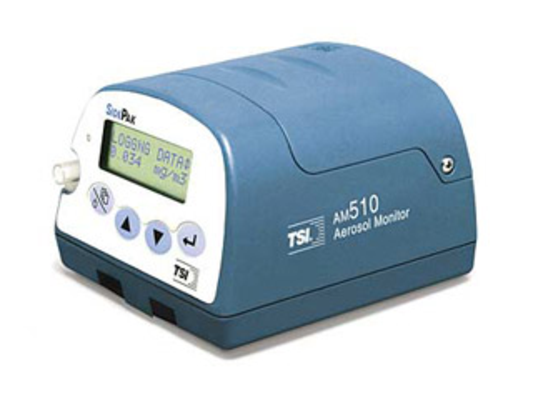
\includegraphics[scale=0.8]{sidepak}
\caption{A TSI-Sidepak for measuring \gls{pm25}}
\label{fig:sidepak}
\end{figure}

According to the TSI website (\cite{TSI2015}), the sidepak is calibrated "\textit{to the respirable fraction of standard ISO 12103-1, A1 Test Dust (formerly Arizona Test Dust) [which] allows comparisons between measurements where the source or type of dust is predominately the same}". Therefore when this device is used it needs calibration factors calculating and applying to the data, to accurately reflect the concentrations in the environment it is recording in. Doing so is relatively simple to do when placed alongside a gravimetric measurement device, and is common in robust studies such as \cite{Torrey2015} where they found the Sidepak was overestimating by a factor of about 1.3 and \cite{Jiang2011} where the Sidepak was overestimating concentrations by a factor of 3. Within London, Dr Barratt has calculated a correction factor of 0.6 for use of the sidepak in outdoor environments (personal communication, 2016). However to our knowledge no correction factor exists for use in the London Underground, and as such this needed calculating. Briefly, as part of a separate research project at \gls{kcl}, a TSI-Sidepak was placed in a small cabin on the platform of Hampstead station (a station on the Northern Line of the network). Alongside this, a ThermoFisher Partisol (\cite{ThermoFisherScientific2016}) was installed and both instruments had inlets pushed through holes in the ceiling of the cabin to sample the air over a three week period. The process and results are described in full in an article which will be submitted in early 2019, but in summary the result was that a correction factor of times two should be applied when the device is sampling \gls{pm25} in the tube. Or rather, this correction should be applied to the proportion of the \gls{pm} that is attributable to the tube, rather than external air (which should have the aforementioned London correction factor of 0.6 applied). This process is illustrated with some simulated data in Figure \ref{fig:tube_correction_example} below.

\begin{figure}[H]
\centering
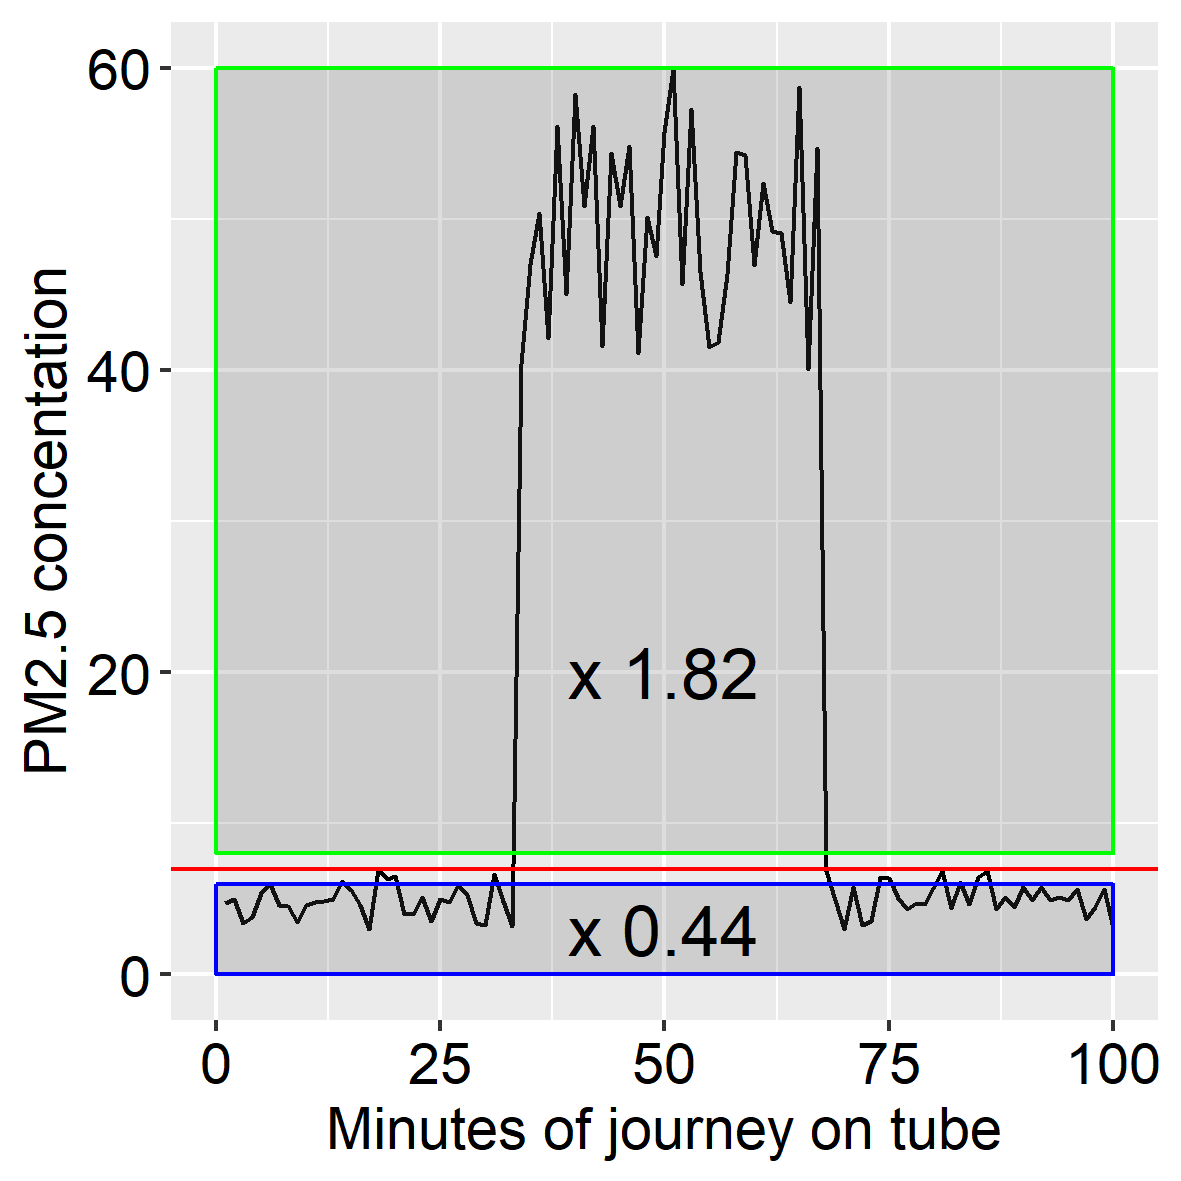
\includegraphics[scale=1]{tube_correction_example}
\caption{Simulated tube data showing the proportion of the data that would be scaled by 2.0 (green box) and the proportion of the data that would be scaled by 0.6 (blue box) if the London background concentration at that time was 7 $\mu \text{g m}^{-3}$ (red line)}
\label{fig:tube_correction_example}
\end{figure}

To apply this scaling factor, the daily average London background concentration of \gls{pm25} was taken from the North Kensington monitoring station (part of the London Air Quality Network (\gls{laqn}) for each of the days that the sampling occurred, and this scaling method was therefore applied to all of the London Underground air quality data presented below.

%%%%%%%%%%%%%%%%%%%%%%%%%%%%%%
\subsection{Tube diary}
\label{tube_diary}
%%%%%%%%%%%%%%%%%%%%%%%%%%%%%%
In order to map \gls{pm25} concentrations across the tube network, location data was needed to combine with the \gls{pm25} data collected by the TSI-Sidepak. Due to around 50\% of the network being underground, where GPS use is not possible, a diary was kept and then transcribed into SQL code, before being loaded into the same database as the Sidepak data. An example of the SQL code is shown below.

\begin{lstlisting}
INSERT INTO tube_diary VALUES('Bakerloo', 'Elephant & Castle', '2015-02-04 08:07:00', '2015-02-04 08:09:00', 'platform', 'floor', 1);
-- Started tube journey North
INSERT INTO tube_diary VALUES('Bakerloo', 'Elephant & Castle', '2015-02-04 08:07:00', '2015-02-04 08:07:00', 'tube', 'shelf', 2);
INSERT INTO tube_diary VALUES('Bakerloo', 'Lambeth North', '2015-02-04 08:13:00', '2015-02-04 08:13:00', 'tube', 'shelf', 3);
INSERT INTO tube_diary VALUES('Bakerloo', 'Waterloo', '2015-02-04 08:15:00', '2015-02-04 08:15:00', 'tube', 'shelf', 4);
INSERT INTO tube_diary VALUES('Bakerloo', 'Embankment', '2015-02-04 08:16:00', '2015-02-04 08:16:00', 'tube', 'shelf', 5);
INSERT INTO tube_diary VALUES('Bakerloo', 'Charing Cross', '2015-02-04 08:17:00', '2015-02-04 08:17:00', 'tube', 'shelf', 6);
INSERT INTO tube_diary VALUES('Bakerloo', 'Piccadilly Circus', '2015-02-04 08:19:00', '2015-02-04 08:19:00', 'tube', 'shelf', 7);
INSERT INTO tube_diary VALUES('Bakerloo', 'Oxford Circus', '2015-02-04 08:21:00', '2015-02-04 08:21:00', 'tube', 'shelf', 8);
\end{lstlisting}

This location data was then linked to the Sidepak data by time and date.

%%%%%%%%%%%%%%%%%%%%%%%%%%%%%%
\subsection{Station and line locations}
%%%%%%%%%%%%%%%%%%%%%%%%%%%%%%
To be able to investigate any spatial patterns in the data collected, we needed to add spatial attributes to the data. Whilst the tube diary and Sidepak data describe in text and numbers that, for example, the \gls{pm25} levels are 37 $\mu \text{g m}^{-3}$ on the stretch of line between Aldgate East and Liverpool Street at 9:32am, we do not have the geographical location of that stretch of track (or indeed the stations at either end). A geographical network of the London Underground was therefore manually created in a PostGIS database. The process is summarised below:

\begin{itemize}
\item Download station locations (latitude/longitude/name) from \gls{tfl} as a \gls{csv} file
\item Compare this list against a tube map to ensure 100\% of stations were present.
\item Identify missing stations (14), use Google Maps to note their lat/long, and add these to the \gls{tfl} \gls{csv}
\item Loaded \gls{csv} into PostgreSQL database
\item Using a printed tube map, make a manual note of each section of track, including the stations that it joins, and the line of the track
\item Digitise this information to a \gls{csv} (start station coordinates, end station coordinates, line ID) and load into PostGIS
\item Use the PostGIS makeline() function to create a linestring feature between each station for each line as appropriate
\item Visualise and error check
\end{itemize}

The key \gls{sql} code to create this is shown in Appendix \autoref{code:make_tube_network_from_scratch}. Loaded into \gls{qgis} for visualisation the network is shown below in Figure \ref{fig:postgis_tube_map}.

\begin{figure}[H]
\centering
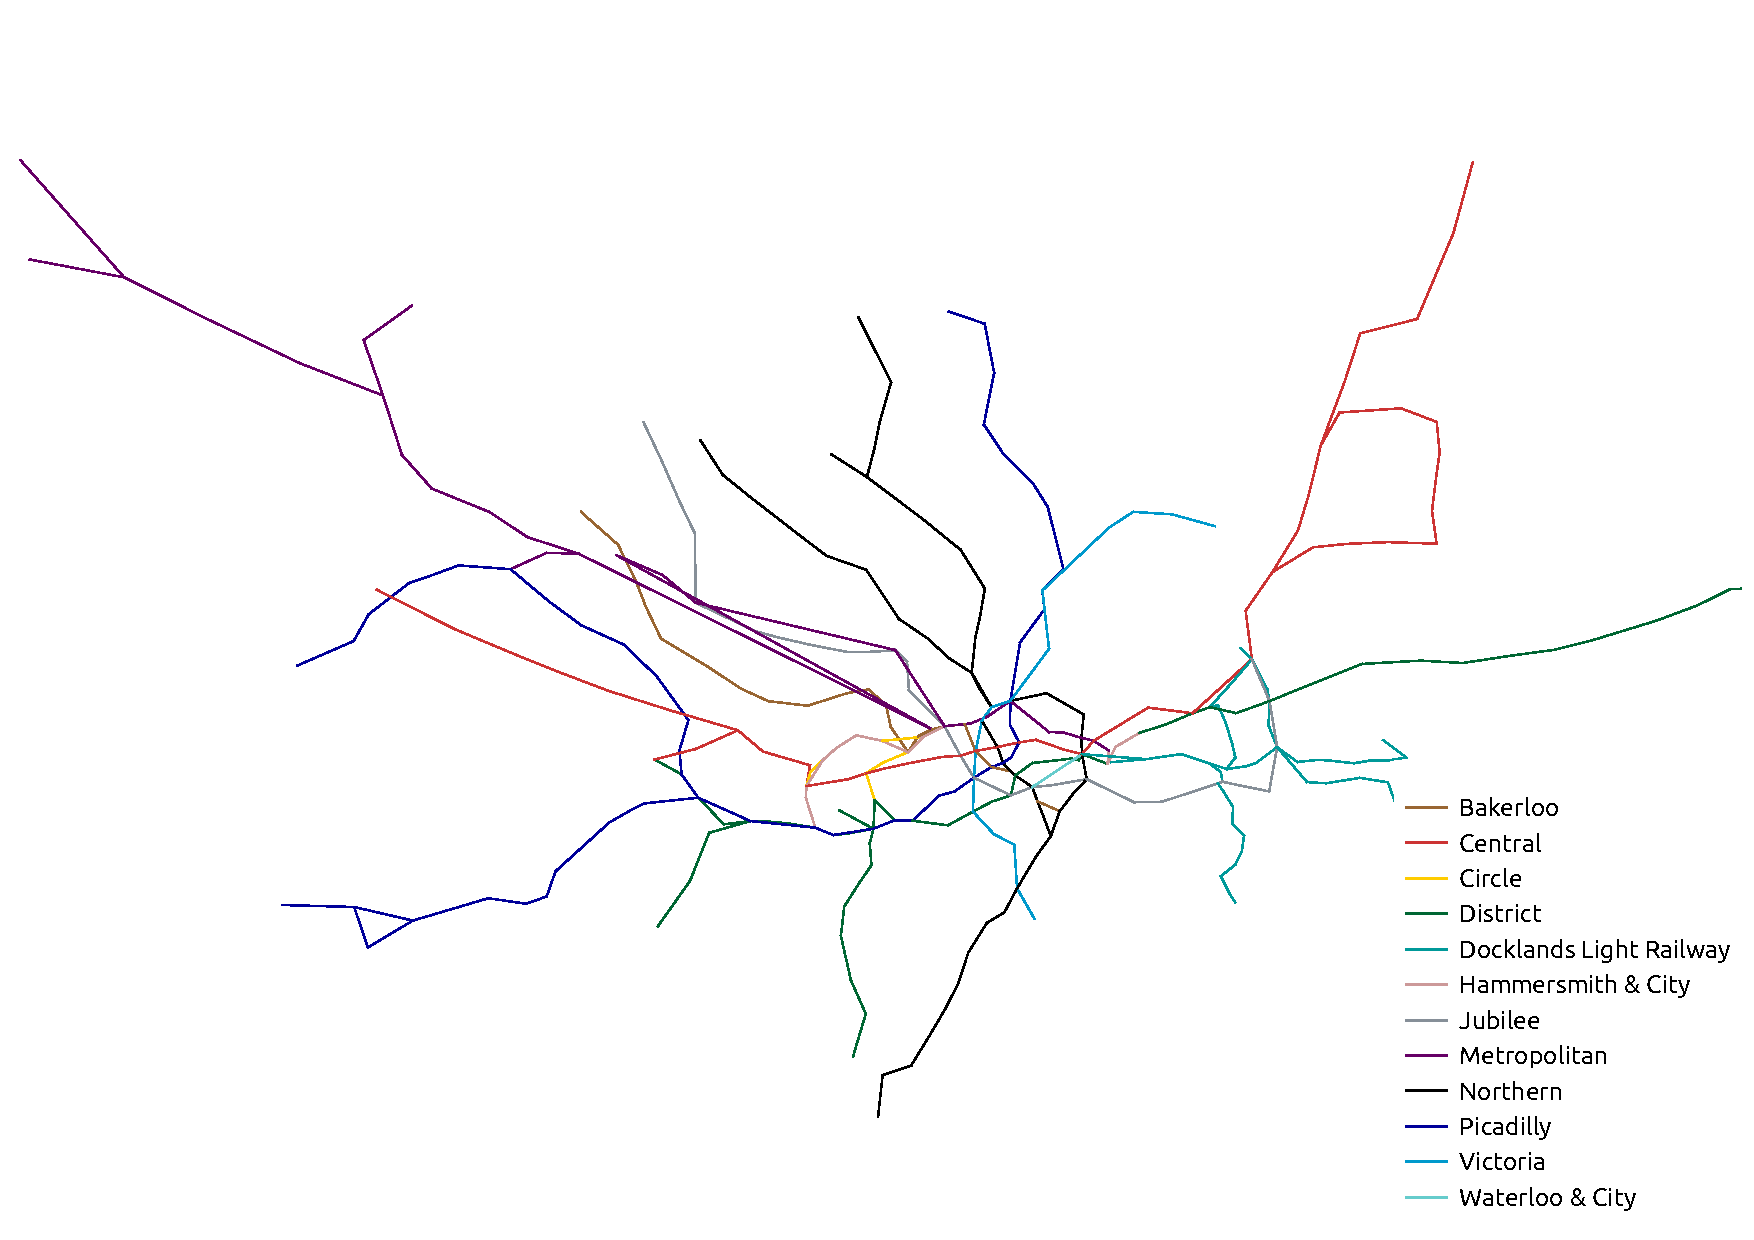
\includegraphics[scale=0.5]{postgis_tube_map}
\caption{PostGIS Tube Map}
\label{fig:postgis_tube_map}
\end{figure}

The map looks different to the traditional London Underground map due to the lines between stations being straight, rather than adjusted for cartographic purposes. The created lines are also not exactly geographically correct, however it was decided that creating a geographically accurate dataset to represent the real-life complexity of the exact routes of the lines was not needed for this work.

%%%%%%%%%%%%%%%%%%%%%%%%%%%%%%
\subsection{London Underground station characteristics}
\label{subsec:station_characteristics}
%%%%%%%%%%%%%%%%%%%%%%%%%%%%%%
As briefly mentioned above, one of my hypotheses is that line and station depths influence \gls{pm25} concentrations on the network. However the data to add a 'z' attribute (depth) of each station was not freely available via the London Datastore or similar official data sources. I was however able to find a Freedom of Information request made by Hamechan Madhoo in January 2013 (\url{https://www.whatdotheyknow.com/request/depth_of_tube_stations_and_tube#incoming-366374}), in which \gls{tfl} provided this data. These data were downloaded, quality checked, errors corrected, and then loaded as a \gls{csv} file into the PostGIS database, and then matched to the existing data by station name and line. Stations on the DLR are all above ground except for Bank, and were missing from this dataset, so for simplicity they were all assigned a depth z value of -10 i.e. 10 metres above ground.

%%%%%%%%%%%%%%%%%%%%%%%%%%%%%%
\subsection{Trains}
\label{subsec:trains}
%%%%%%%%%%%%%%%%%%%%%%%%%%%%%%
Data regarding the types of trains that are operated on each line was also sourced from from the \gls{tfl} website (\cite{TransportforLondon2016}), thinking it might be useful, and is summarised in Table \ref{tab:train_type_on_the_underground} below.


\begin{table}[H]
\caption{Train type running on each tube line}
\centering
    \begin{tabular}{ | l | l | l |}
    \hline 
     \bfseries{Line} & \bfseries{Train}             \\ \hline
        Victoria                &   2009 stock      \\ \hline
        Circle                  &   'S' stock (2010)       \\ \hline
        Northern                &   1995 stock      \\ \hline
        Bakerloo                &   1972 stock      \\ \hline
        Jubilee                 &   1996 stock      \\ \hline
        District                &   'D' stock (1980)      \\ \hline
        Piccadilly              &   1973 stock      \\ \hline
        Docklands Light Railway &   'B07' stock (2005)     \\ \hline
        Metropolitan            &   'S' stock (2010)       \\ \hline
        Central                 &   1992 stock      \\ \hline
        Hammersmith \& City     &   'S' stock (2010)       \\ \hline
        \end{tabular}
\label{tab:train_type_on_the_underground}
\end{table}

%%%%%%%%%%%%%%%%%%%%%%%%%%%%%%
\section{Results}
\label{sec:3results}
%%%%%%%%%%%%%%%%%%%%%%%%%%%%%%

%%%%%%%%%%%%%%%%%%%%%%%%%%%%%%
\subsection{Timeline concentrations}
\label{subsec:timeline_concentrations}
%%%%%%%%%%%%%%%%%%%%%%%%%%%%%%

To gain an initial understanding of the concentrations and variation between each line, a time-line graph of all the data was created (Figure \ref{fig:all_lines_pm25}). The x axis was taken as minutes on the line, hence the lines that had more monitoring completed on them (sometimes due to the length of the line, sometimes due to availability of the researcher) continue further to the right of the graph than others, noting that there were repeats of each line section.

\begin{figure}[H]
\centering
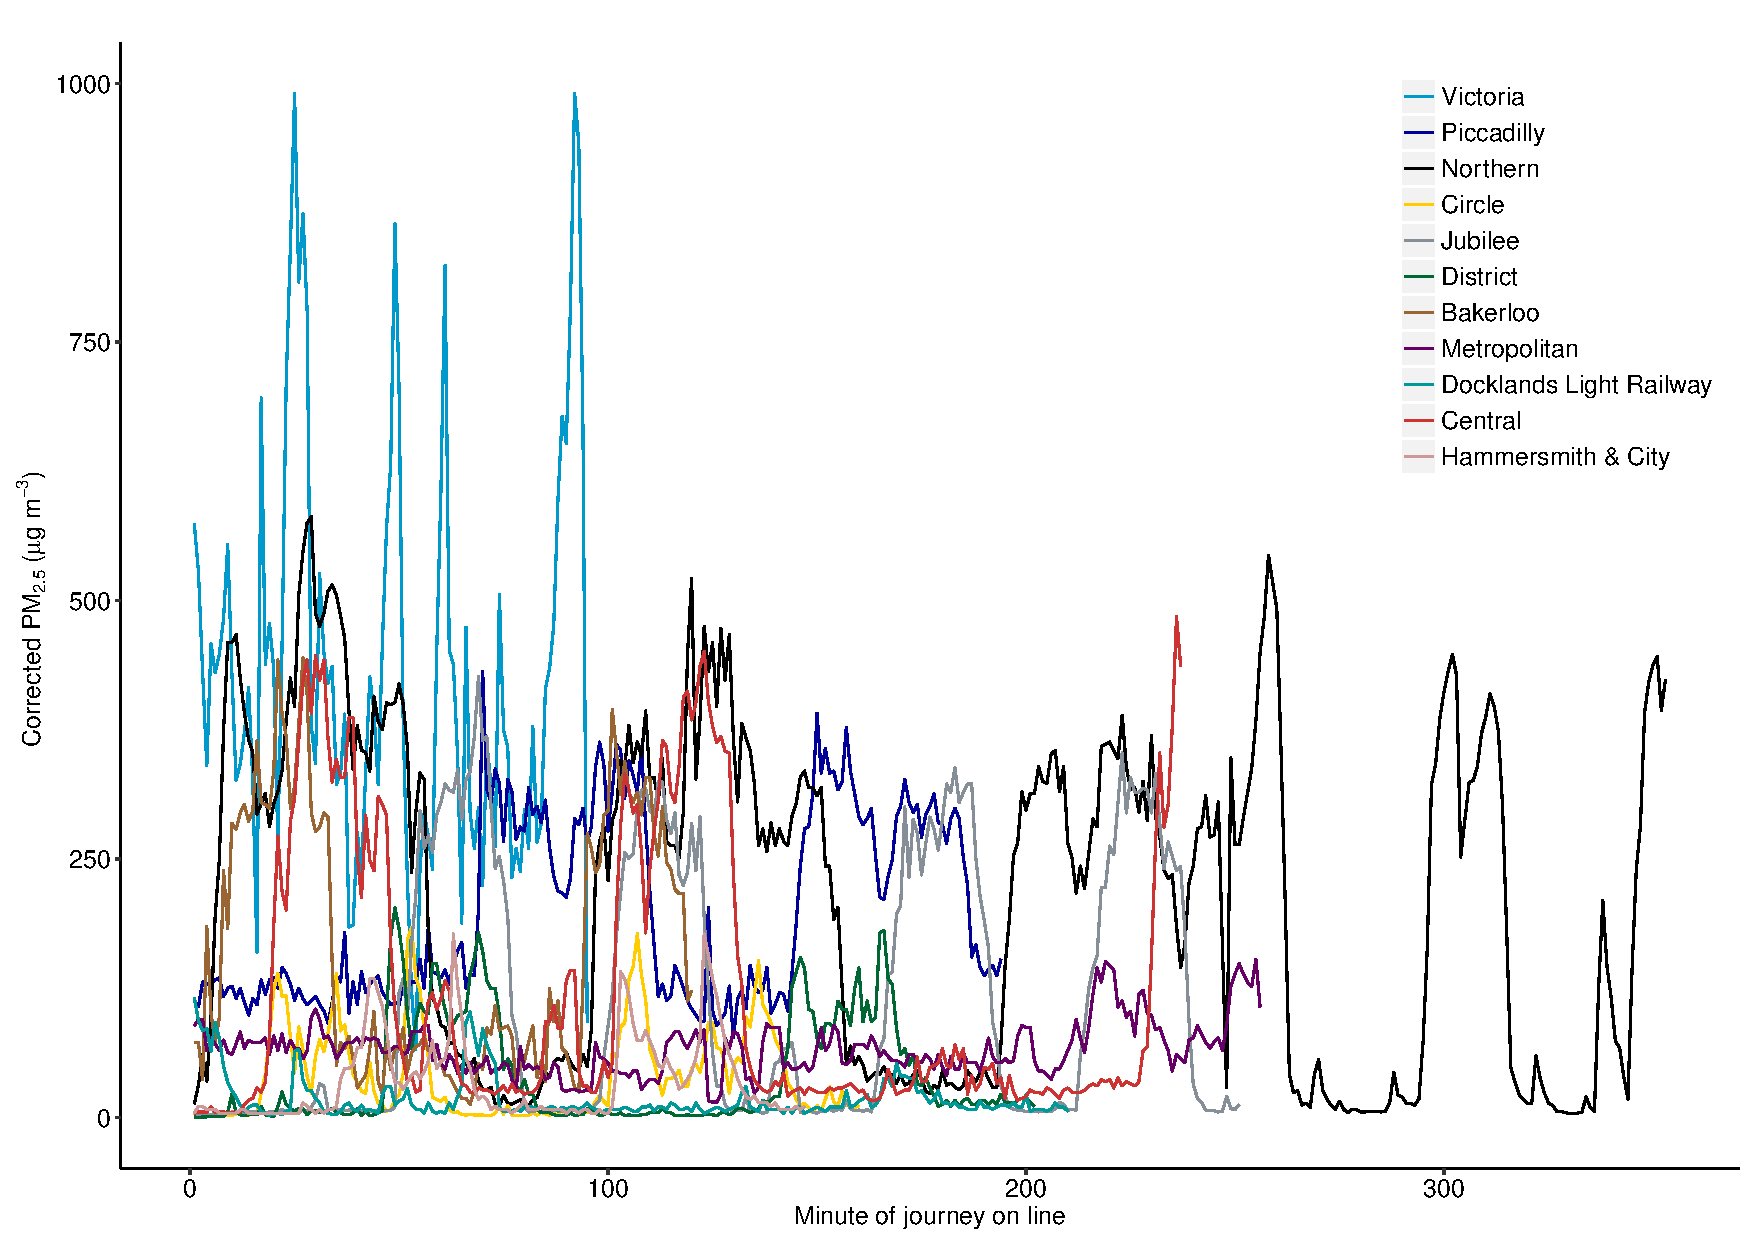
\includegraphics[scale=0.5]{all_lines_pm25}
\caption{Timelines of \gls{pm25} on the tube}
\label{fig:all_lines_pm25}
\end{figure}

Although plotting all the lines on top of each other in this way makes the data hard to interpret, it does immediately show the large variation in some lines, and the lack of variation in others. There are clear peaks and troughs, most apparent in the Northern line data, compared to the DLR or Metropolitan lines which although still have variation, the scale is much smaller. Figure \ref{fig:all_lines_individual_pm25_p1} below plots the lines individually to enable better understanding of the patterns.

\begin{figure}[H]
\centering
\caption{Timelines of \gls{pm25} on the tube (Note differing axis scales)}
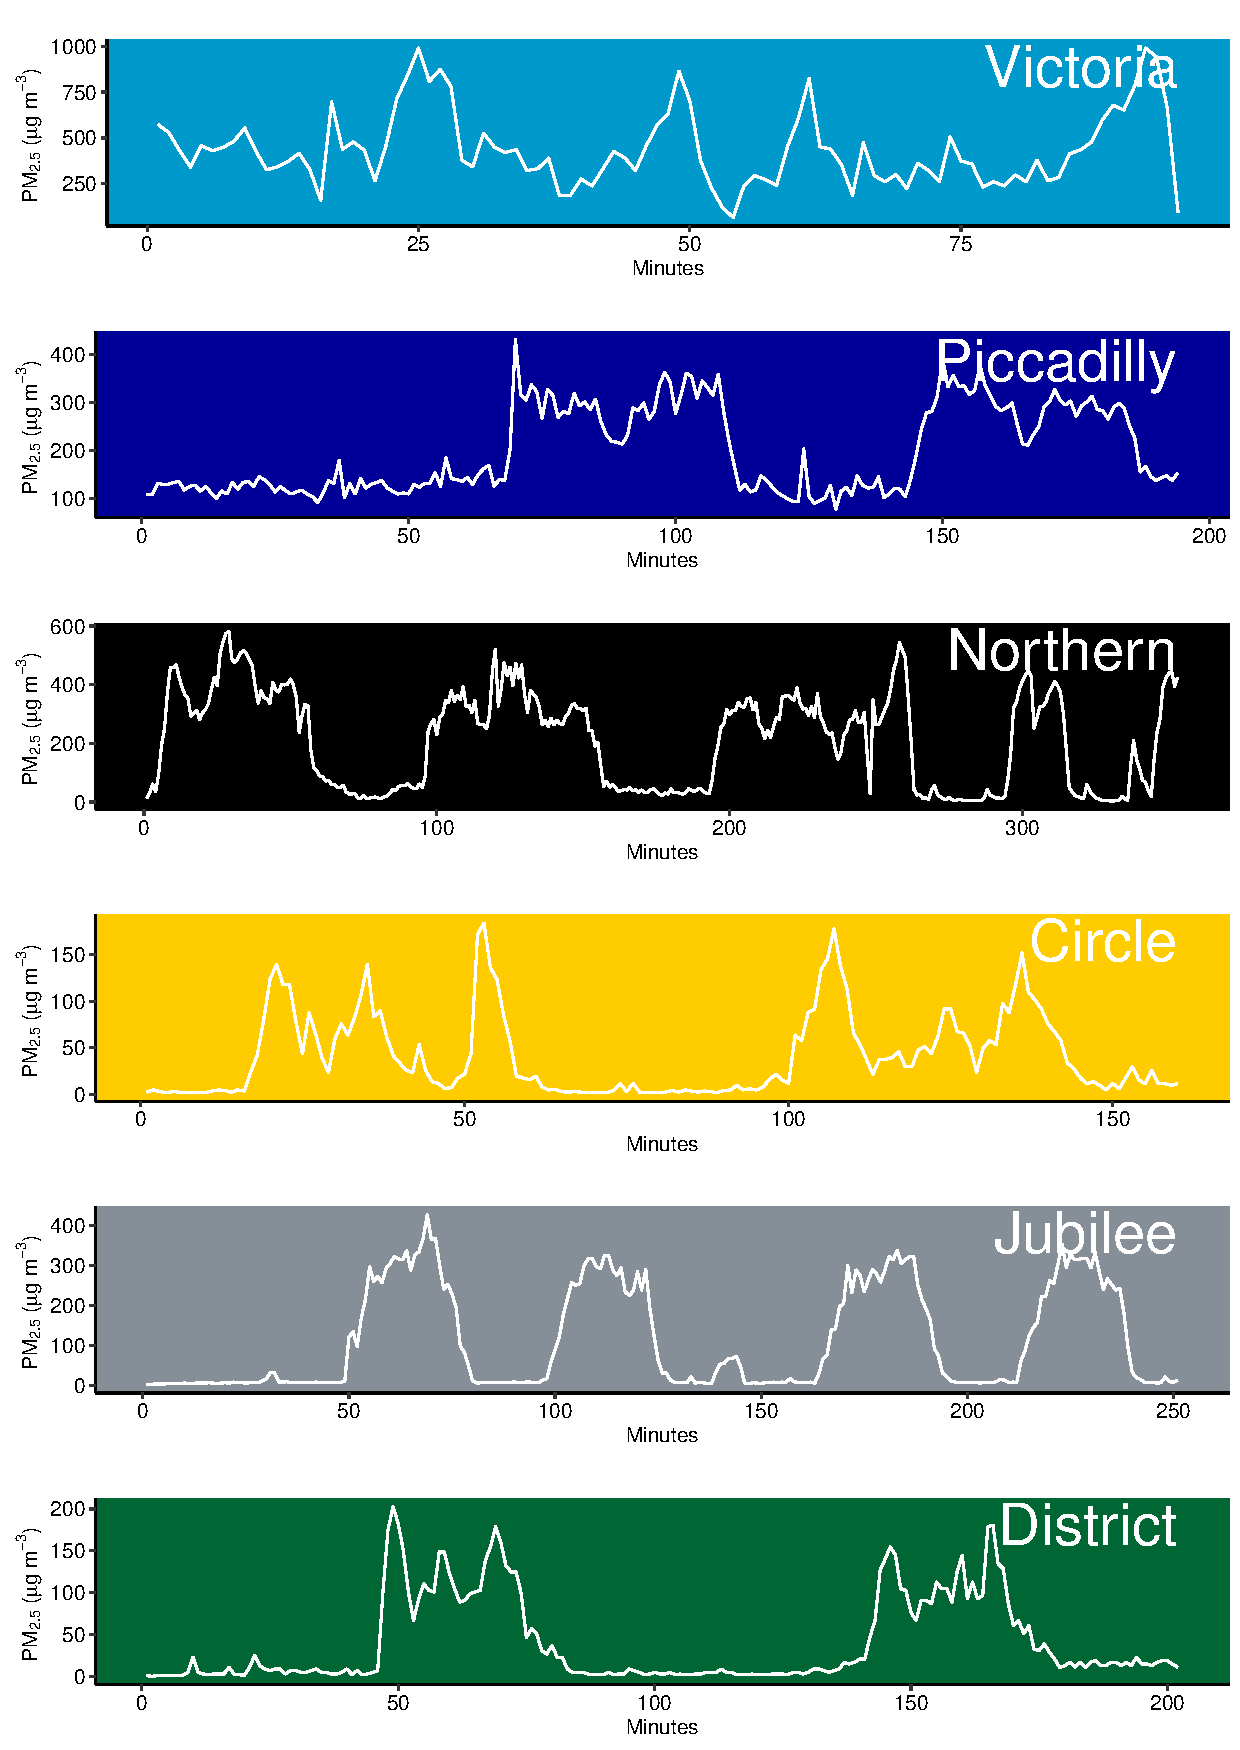
\includegraphics[scale=0.8]{all_lines_individual_pm25_p1}
\label{fig:all_lines_individual_pm25_p1}
\end{figure}

\begin{figure}[H]
\centering
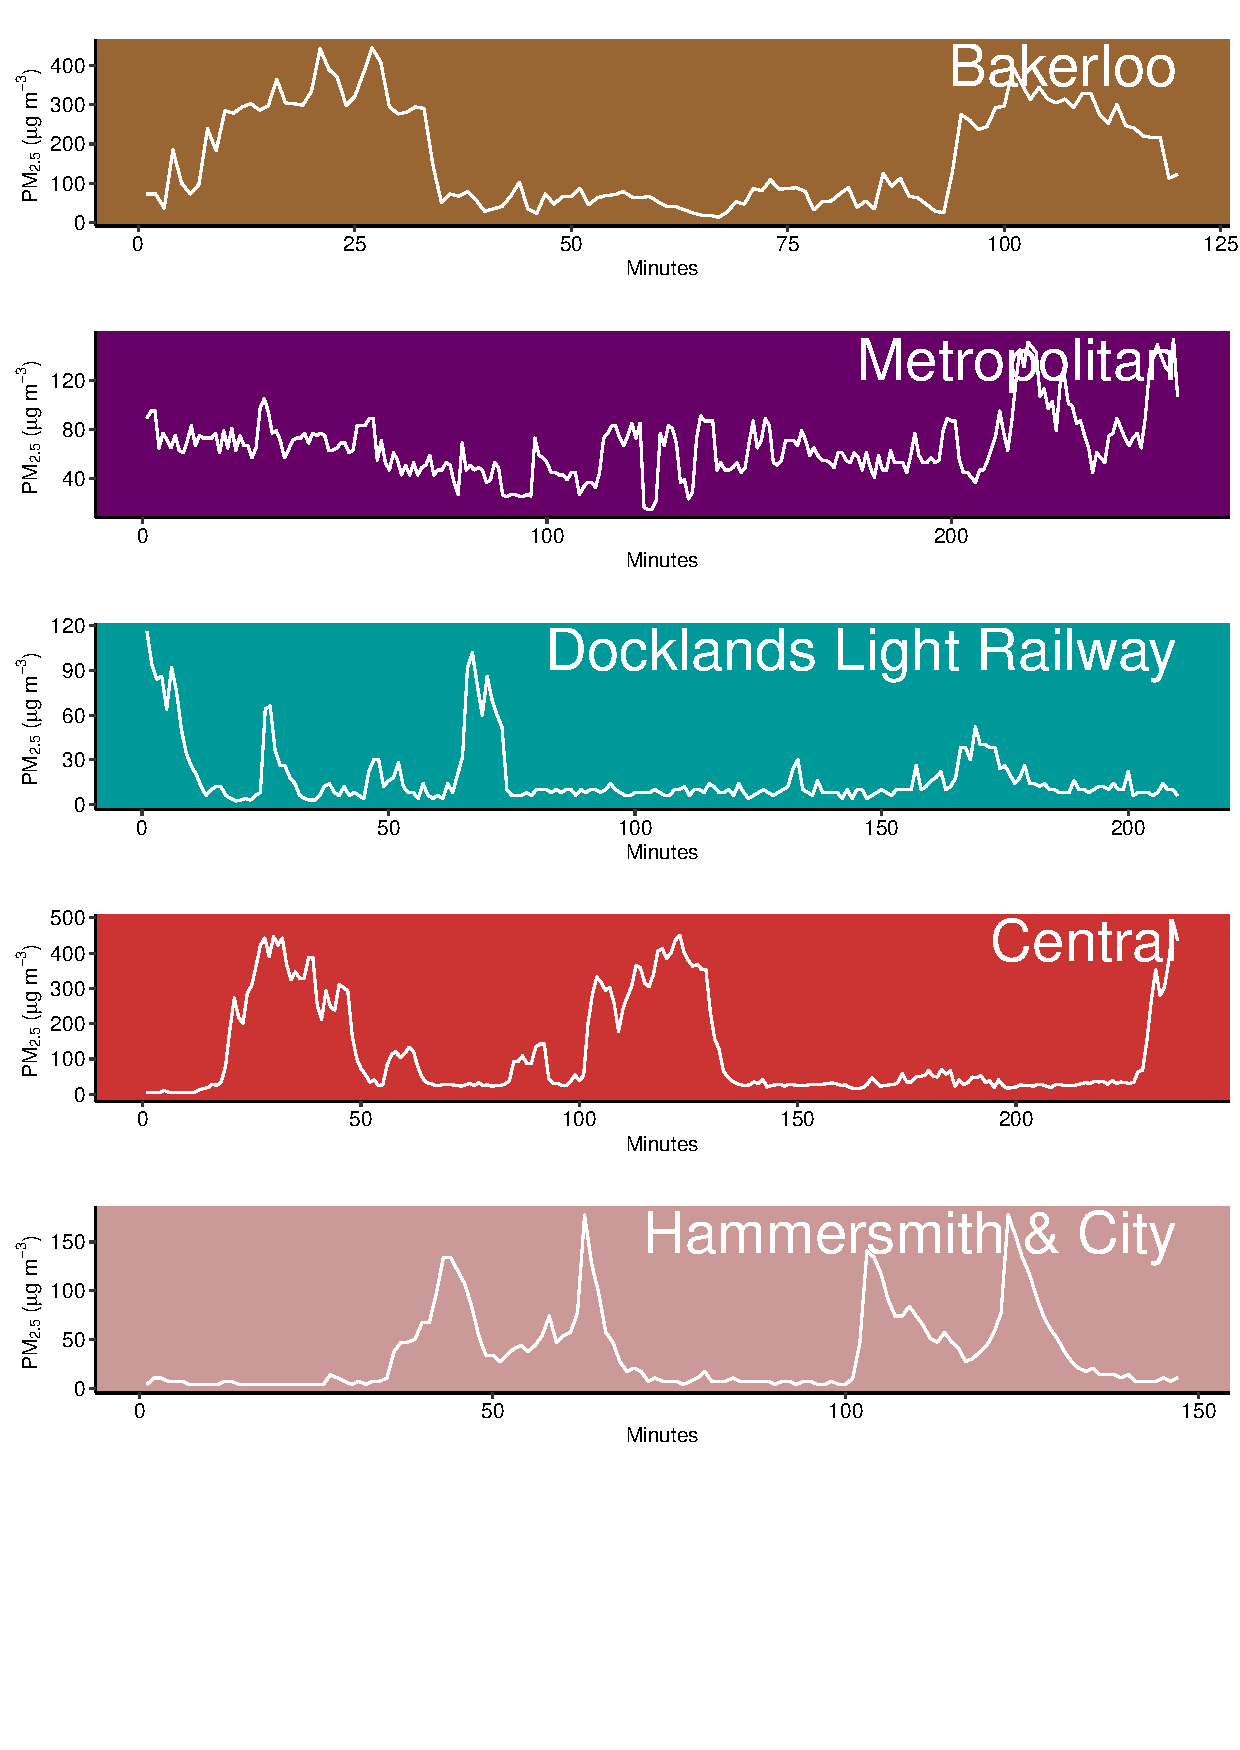
\includegraphics[scale=0.8]{all_lines_individual_pm25_p2}
\label{fig:all_lines_individual_pm25_p2}
\end{figure}

We can see that the concentrations vary by line and within lines, for example the Hammersmith \& City line has a maximum of around 170 $\mu \text{g m}^{-3}$, compared to lines such as the Central line with concentrations upto 500 $\mu \text{g m}^{-3}$ and the Victoria line of upto 900 $\mu \text{g m}^{-3}$. Additionally, for some of the lines, there are clear patterns in the data. The Jubilee line has four clear peaks, and similarly the District line two clear peaks. Referencing these against the diary information that was collected, the peaks coincide with the train being underground, and then 'flat' low levels of \gls{pm25}, when the train was above ground and exposed to ambient air.

%%%%%%%%%%%%%%%%%%%%%%%%%%%%%%
\subsection{Line averages}
\label{subsec:line_averages}
%%%%%%%%%%%%%%%%%%%%%%%%%%%%%%

Box and whisker plots using the ggplot2 package of R (\cite{ggplot2}) were created in Figure \ref{fig:boxplot_pm25_lines} to compare concentrations between lines. 

\begin{figure}[H]
\centering
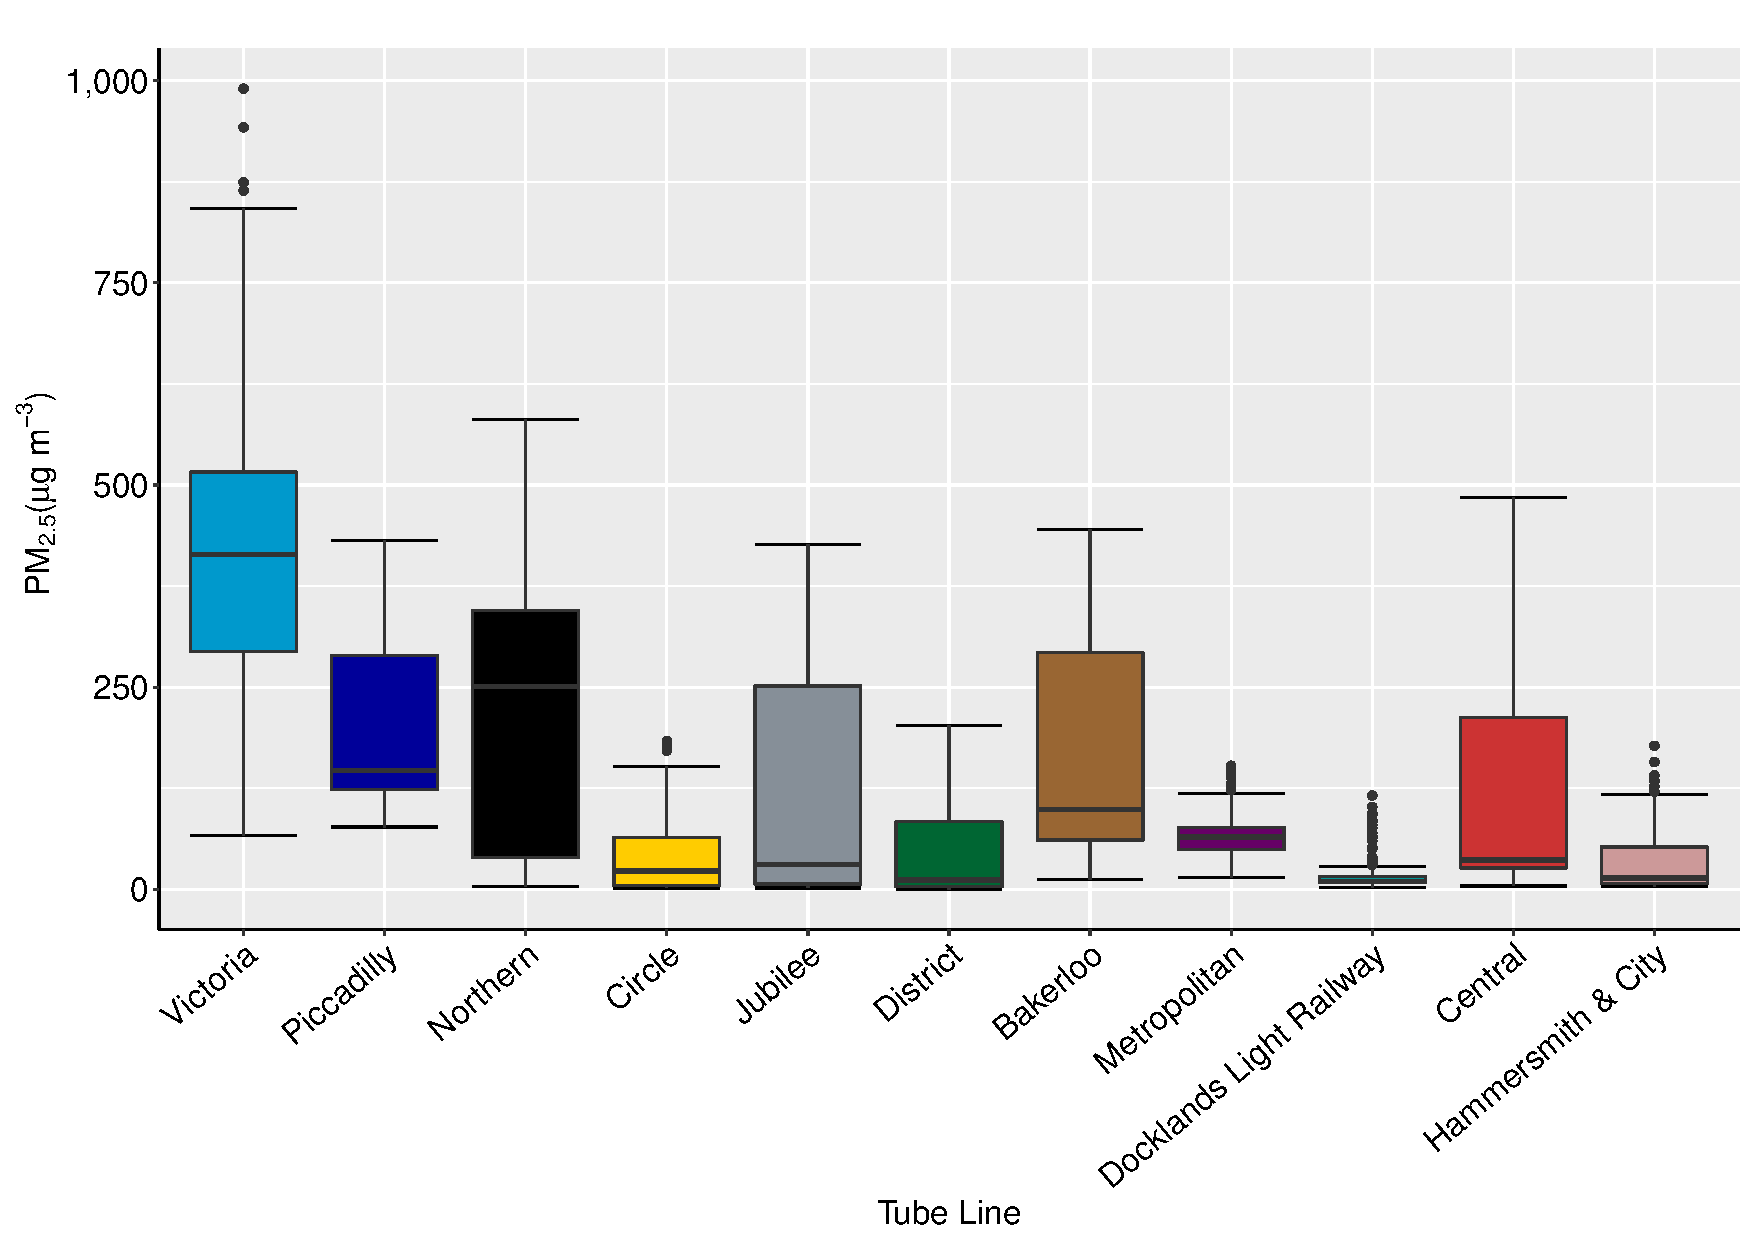
\includegraphics[scale=0.55]{pm25_on_underground}
\caption{PM${2.5}$ $\mu \text{g m}^{-3}$ on the tube, summarised by line. The lower and upper hinges correspond to the 25th and 75th percentiles, the horizontal line to the median, and the whiskers to 1.5 x the inter-quartile-range (approx. 95\% percentile).}
\label{fig:boxplot_pm25_lines}
\end{figure}

This visualisation gives a much clearer picture of the concentrations and variations found between lines, and although the boxplot has identified a number of concentrations on each line as outliers, it is worth noting that this is likely not representative of bad data or device error, it is actually that there are a number of places on some of the lines with substantially higher concentrations that the median. This is most apparent with the Victoria Line where there are concentrations recorded of over 900  $\mu \text{g m}^{-3}$ compared to the median of around 280  $\mu \text{g m}^{-3}$. Interestingly the Circle, District, Metropolitan, Docklands Light Railway, and Hammersmith \& City lines all have noticeably lower medians than the other lines and a relatively small inter-quartile range. Given that the environment of the tube varies between fully exposed to the outside air (in the manner of a normal train), to semi-covered, to fully underground, it seems a reasonable premise that these different environments are effecting the rises and falls in concentrations as per the timelines in Figure \ref{fig:all_lines_individual_pm25_p1}. This was tested in Section \ref{subsec:concentrations_v_depth}.

%%%%%%%%%%%%%%%%%%%%%%%%%%%%%%
\subsection{Concentrations v. Depth}
\label{subsec:concentrations_v_depth}
%%%%%%%%%%%%%%%%%%%%%%%%%%%%%%

To compare concentrations by line, the mean station depth of all stations on a line was calculated and plotted against the mean \gls{pm25} concentration for that line (Figure \ref{fig:concentrations_depth_summary})

\begin{figure}[H]
\centering
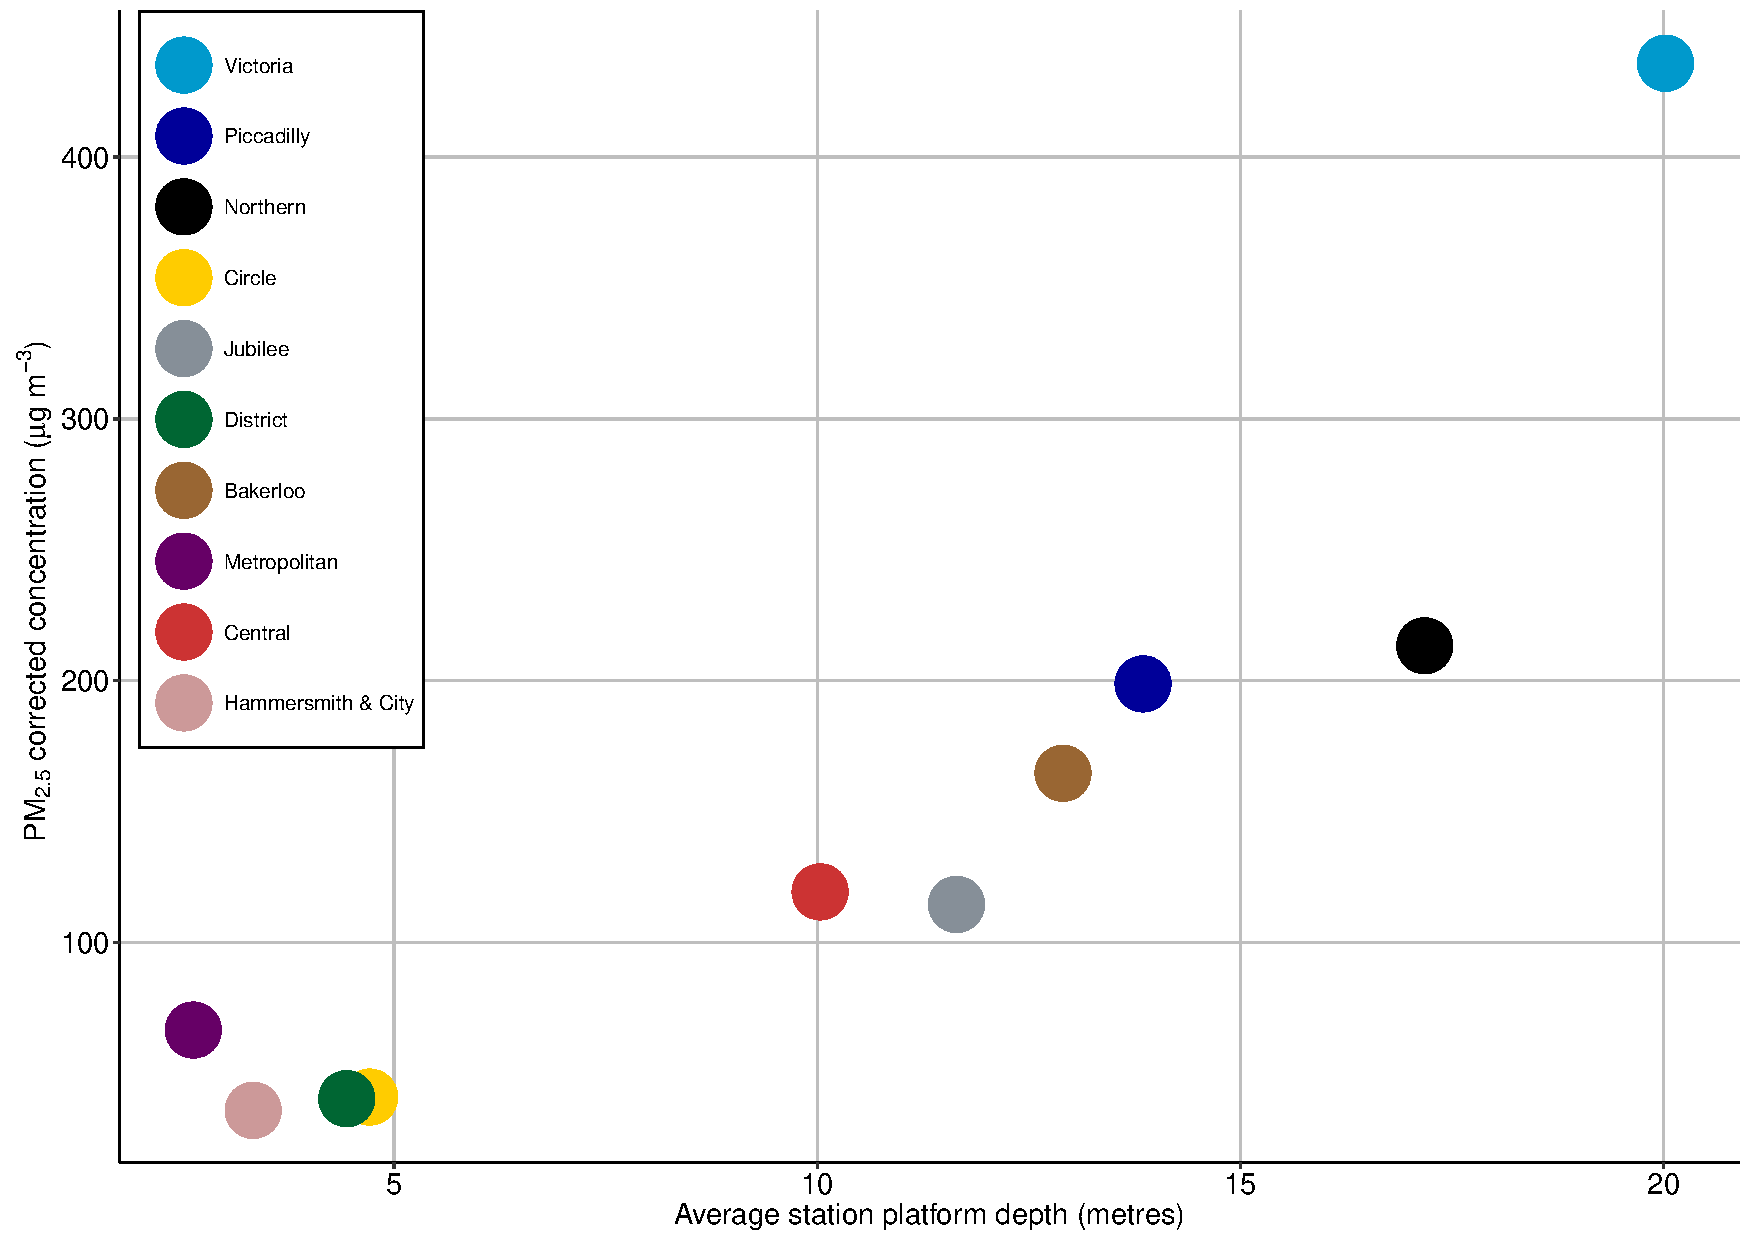
\includegraphics[scale=0.55]{depth_pm25_summary}
\caption{Mean concentrations v. mean station depths by tube line}
\label{fig:concentrations_depth_summary}
\end{figure}

Plotting the average line depths against average line concentrations appears to back-up that depth is an important determinant of levels of \gls{pm25}. The shallower lines have the lowest average concentrations, and the deepest lines the highest. To explore this further, figure \ref{fig:depth_plot_per_line_pm25} plots the concentrations for each station of each line in the same manner. Each point is the mean of the \gls{pm25} concentrations recorded at that station.

\begin{figure}[H]
\centering
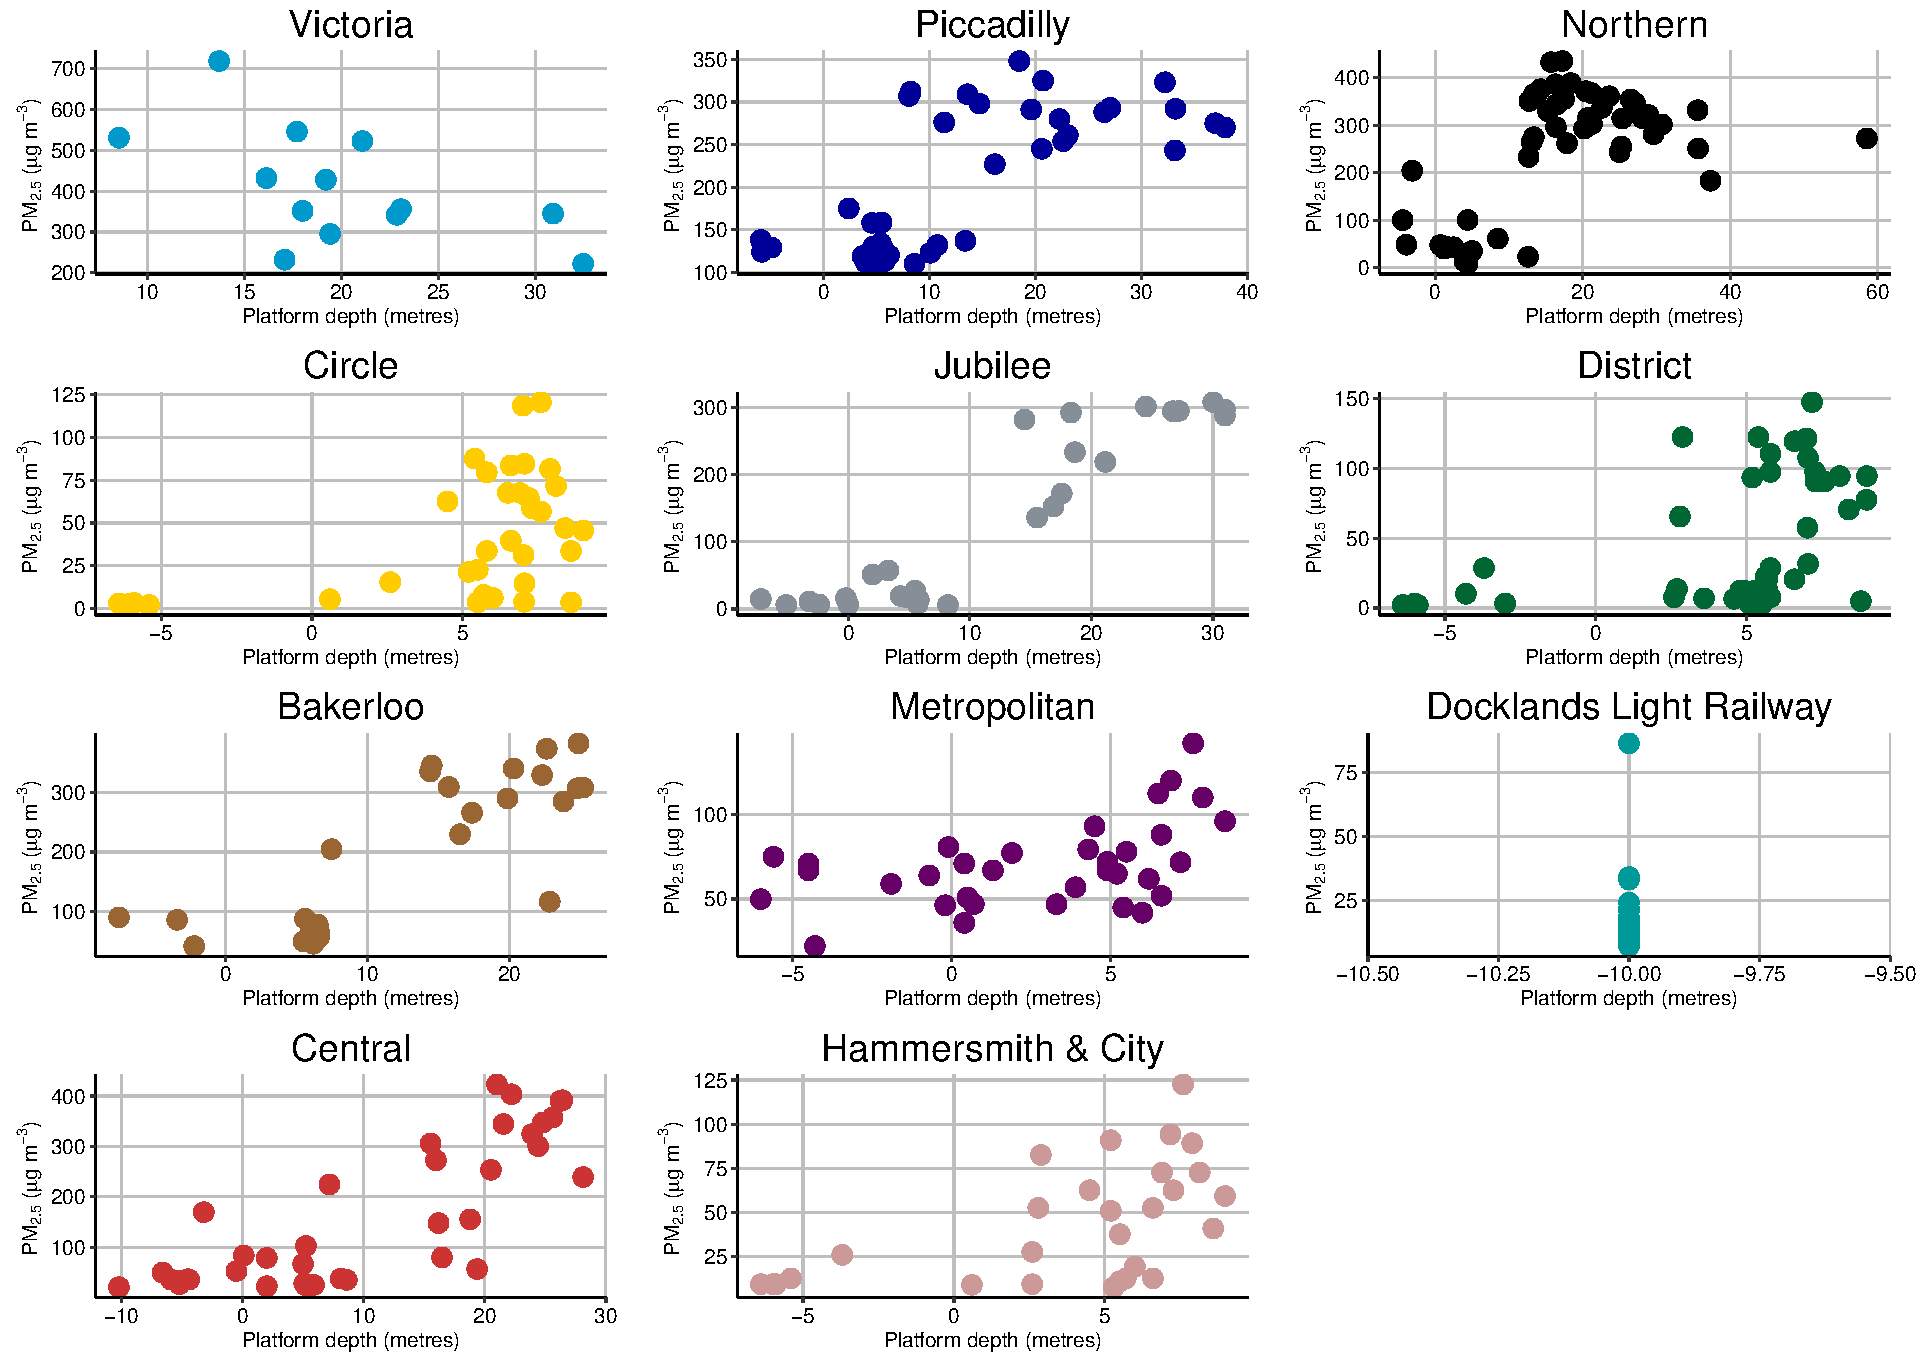
\includegraphics[scale=0.5]{depth_plot_per_line_pm25}
\caption{Concentrations recorded at stations v. station depth}
\label{fig:depth_plot_per_line_pm25}
\end{figure}

The relationship between depth and concentrations that was apparent in Figure \ref{fig:concentrations_depth_summary} is not so clear in Figure \ref{fig:depth_plot_per_line_pm25}, i.e., once the depth and concentrations are plotted for each individual station as opposed to a line average. Although there still seems to be a relationship between depth and \gls{pm25}, it does not seem to be such a straight-forward relationship as increasing depth equals increasing concentrations. Taking the District line as an example (Figure \ref{fig:depth_plot_district_line}), the stations mostly either have a depth of 5 metres above ground, or 5 metres below ground. The stations above ground ($<0$ metres) tend to have low concentrations, but the stations below ground ($>0$ metres) have both high and low concentrations (highlighted with black and blue boxes below in Figure \ref{fig:depth_plot_district_line}).

\begin{figure}[H]
\centering
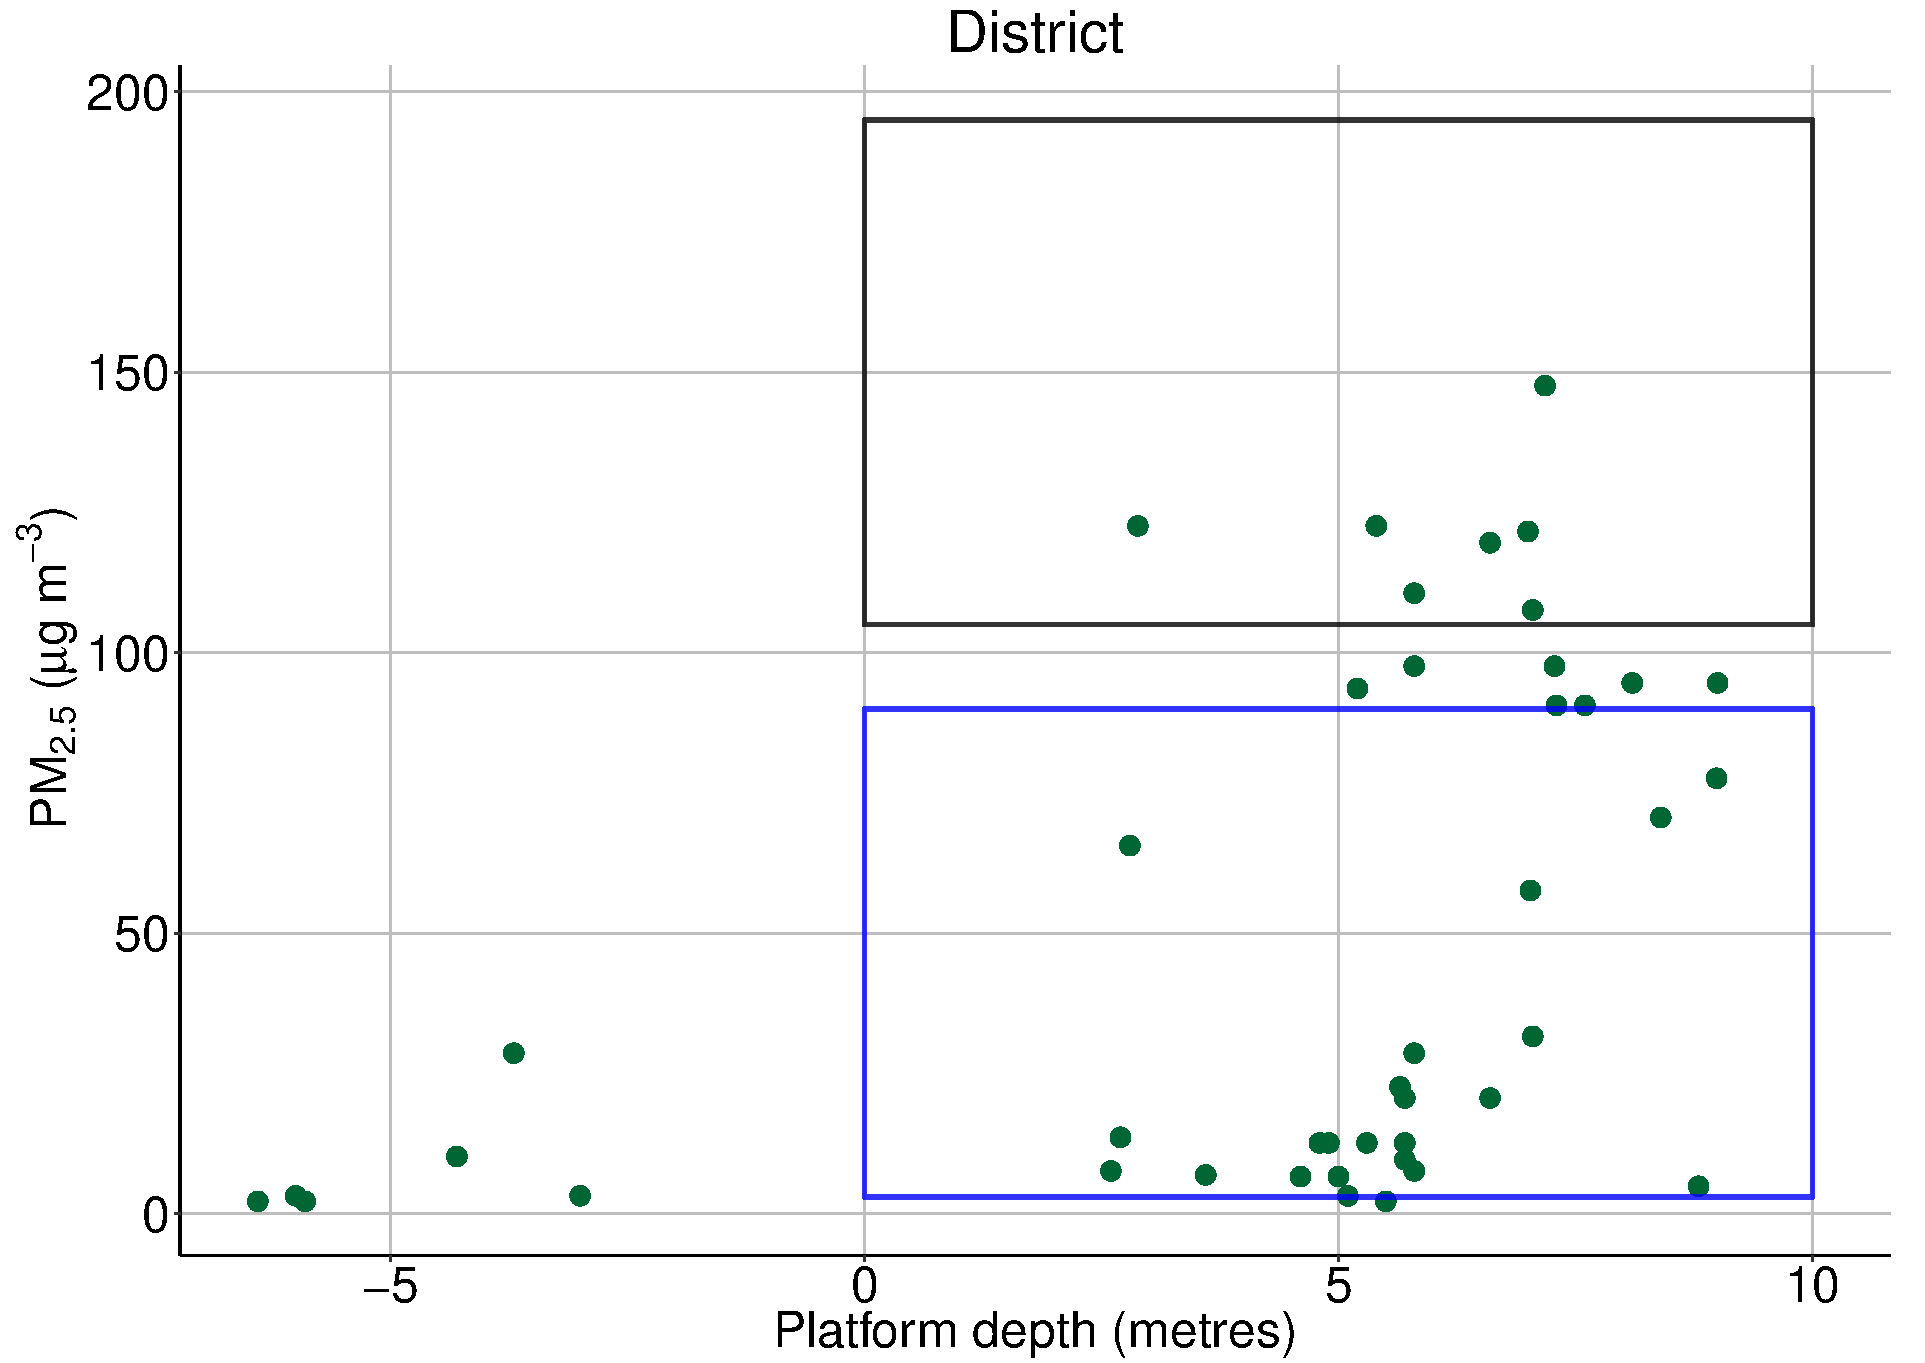
\includegraphics[scale=0.4]{depth_plot_district_line}
\caption{Concentrations recorded at District line stations v. station depth}
\label{fig:depth_plot_district_line}
\end{figure}

Similarly taking the Central line (Figure \ref{fig:depth_plot_central_line}), there is a general increase in \gls{pm25} as station depth increases, except for Gants Hill and Wanstead. These two stations have a depth of 18-20 metres, but concentrations of only 100 $\mu \text{g m}^{-3}$, unlike other stations with similar depths where \gls{pm25} is in the range 300-500 $\mu \text{g m}^{-3}$ (marked with a black box).

\begin{figure}[H]
\centering
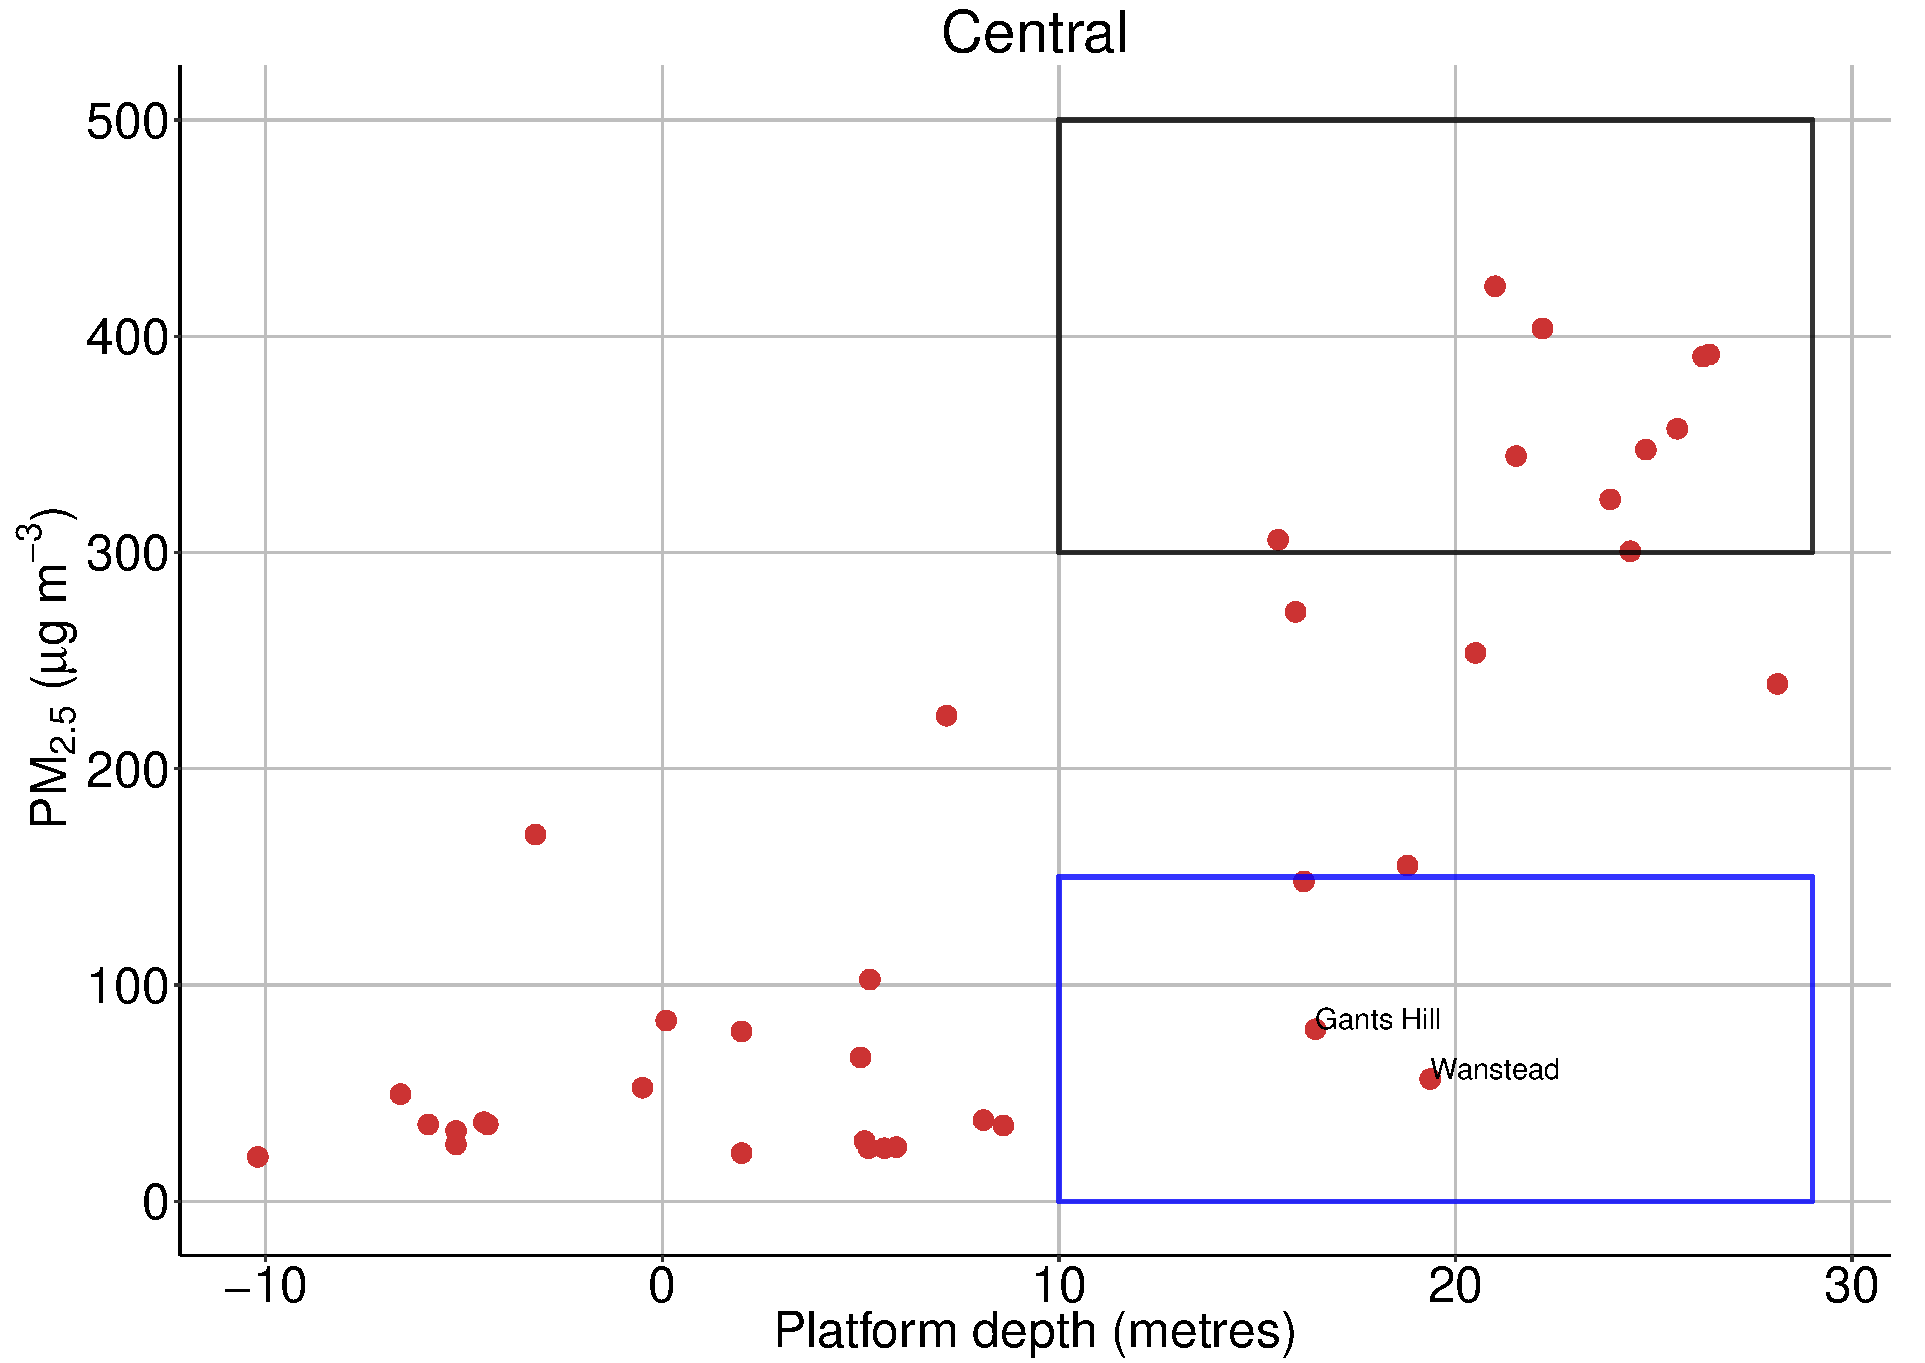
\includegraphics[scale=0.4]{depth_plot_central_line}
\caption{Concentrations recorded at Central line stations v. station depth}
\label{fig:depth_plot_central_line}
\end{figure}

Manually inspecting the depths of Wanstead and Gants Hill, and the stations before and after them on the line, it becomes clear that these stations are in an area of the Central line network where stations are mostly shallow, and that these two are an exception. This could mean that shallow stations tend to be more well ventilated due to natural air circulation, and that this cleaner air is being moved down the tunnels to Gants Hill and Wanstead by the movement of the train, or indeed that the train cabin is being 'flushed' with cleaner air at those station platforms and that it does not build back up to higher concentrations by only going one stop. A plot of the geography of the line, along with concentrations and depth was made in Figure \ref{fig:fake_central_line_pm25} to better understand this point (Code for creation in \ref{code:fake_tube_map_central_line}).

\begin{figure}[H]
\centering
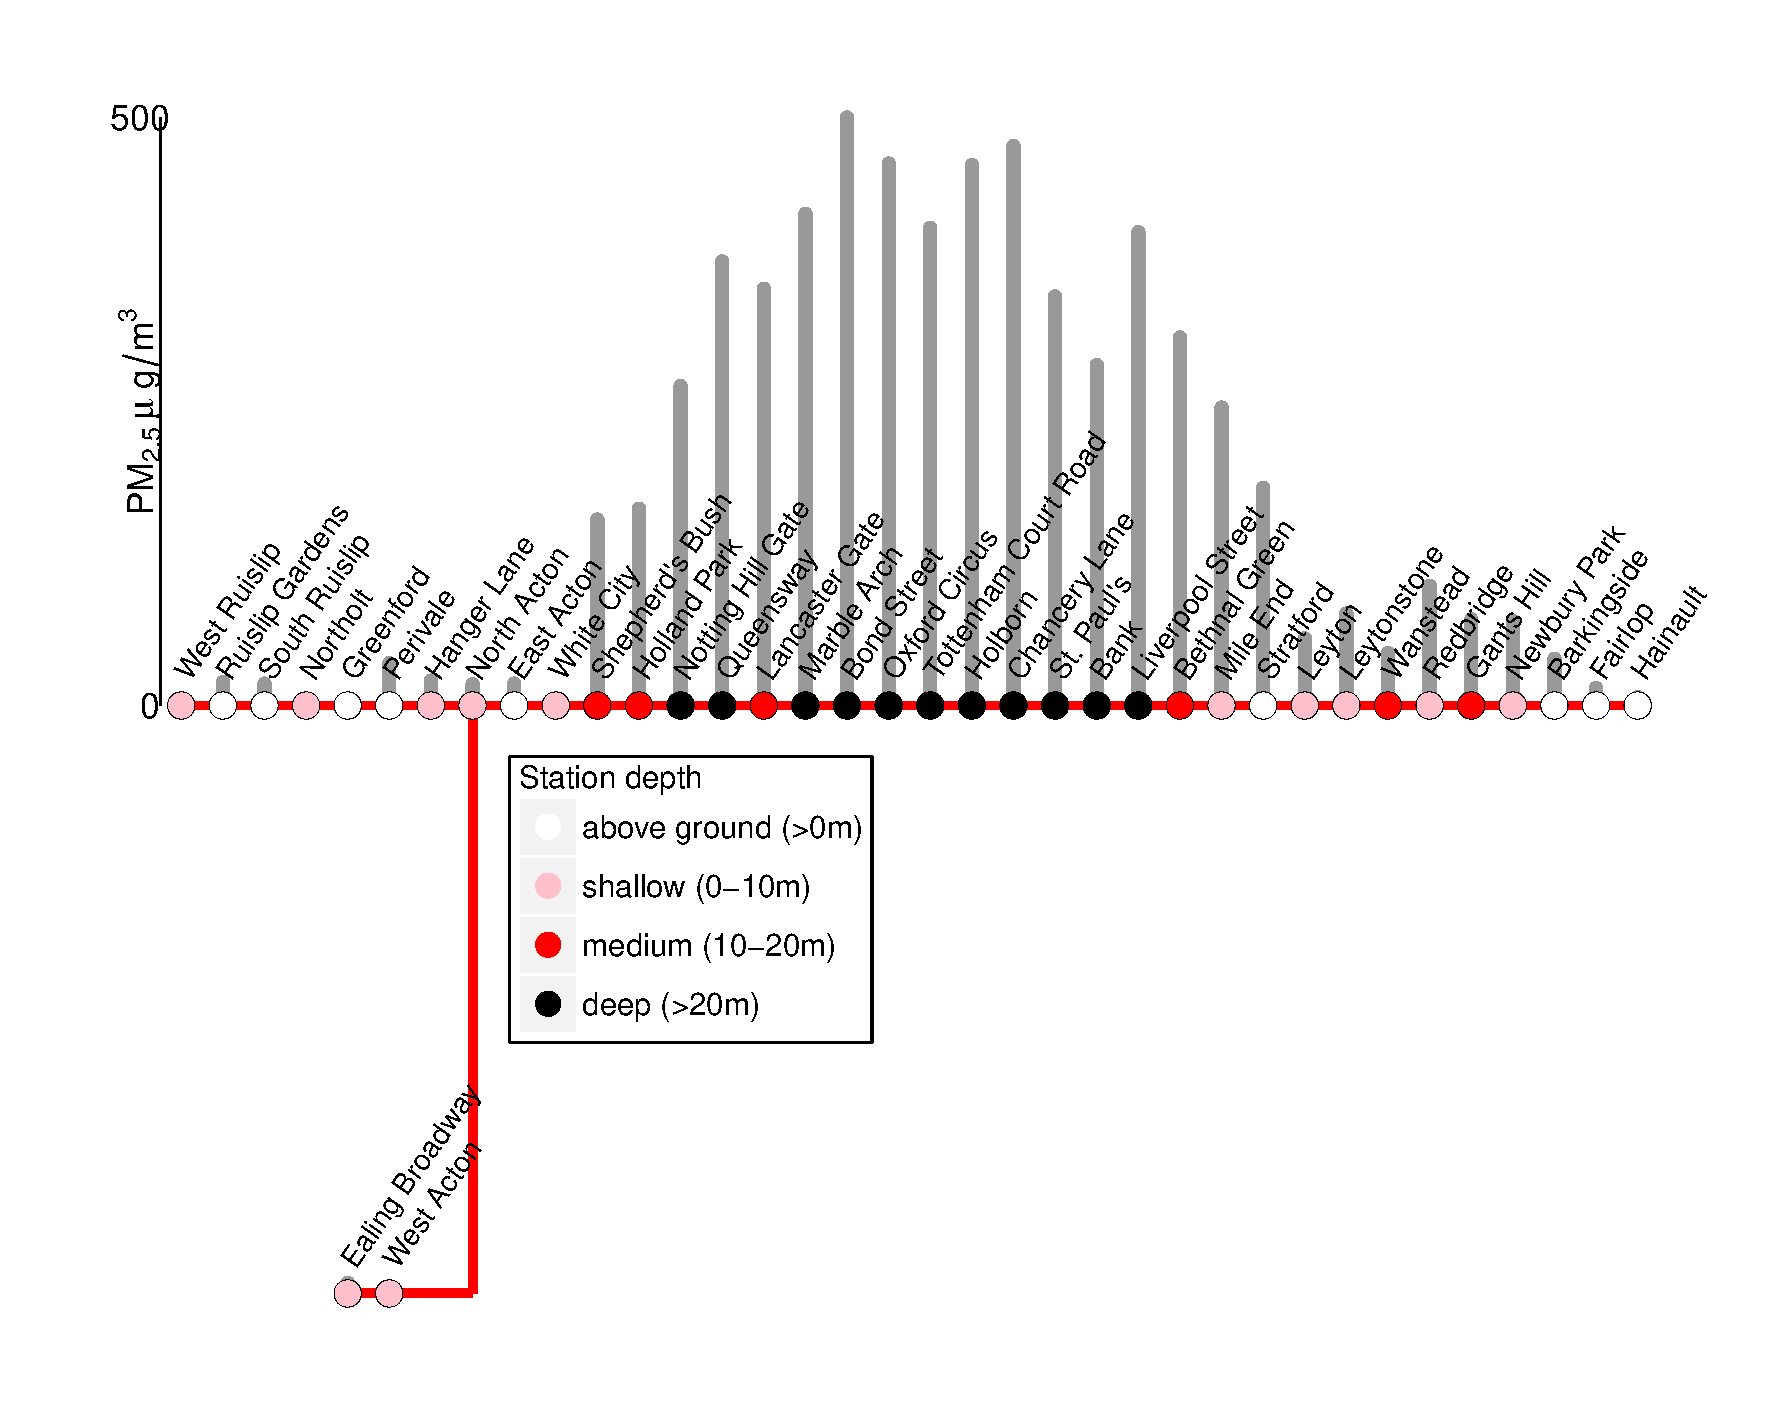
\includegraphics[scale=0.45]{fake_central_line_pm25}
\caption{Central line locations, depths and \gls{pm25}}
\label{fig:fake_central_line_pm25}
\end{figure}

From the plot we can see that Wanstead and Gants Hill (towards the right of the graph) are both medium depth stations (shown as red circles), and as such might be expected to have pollutant concentrations similar to other medium depth stations such as Shepherd's Busy, Holland Park, Bethnal Green and Lancaster Gate. But the \gls{pm25} levels are actually more like that of above ground and shallow stations, suggesting that the depth of a station is not directly related to \gls{pm25} concentrations, and that distance from outdoors or shallower stations is important too.

Taking a further example of stations and concentrations that do not seem to fit the pattern of deep equals high, and shallow equals low, Golders Green has a depth of less than 0, i.e. above ground, but concentrations of over 200 $\mu \text{g m}^{-3}$. From manual inspection of the data, this station is located on the North-West spur of the Northern end of the Northern line. The mean value for the station of 200 $\mu \text{g m}^{-3}$ is calculated as an average of four four recorded values; 356 $\mu \text{g m}^{-3}$, 14 $\mu \text{g m}^{-3}$, 374 $\mu \text{g m}^{-3}$ and 74 $\mu \text{g m}^{-3}$. Looking at this data in more detail, the higher two recorded concentrations relate to the train arriving at Golders Green having just emerged from the tunnel and deep station of Hampstead, and the lower concentrations are when the train has arrived from East Finchley (an above ground station further North on the track). The difference in these values is quite extreme and suggests that for stations that are outside or shallow, but close to deeper stations, the direction of travel influences the \gls{pm25} concentrations for that location. As the tube train arrives at Hampstead from within the deep tunnels further South, the carriage must still be full of air that has accumulated over the journey, which will get partly flushed out by the doors opening at Golders Green, but not before the Sidepak device (with one minute resolution) has recorded high concentrations 'at' Golders Green, which then drop by the next station at East Finchley. Conversely, when the tube arrives at Golders Green from East Finchley, the air inside the carriage is much cleaner as it has not been deep underground previously. The concentrations inside the carriage only start to rise to levels of 200 - 400 $\mu \text{g m}^{-3}$ once tube has gone into the tunnel at Hampstead and started to be exposed to the higher concentrations found in those deeper tunnels. 

To further explore this pattern, the data for Oxford Circus on the Victoria line was examined. There were four measurements taken while on the train at that station, which were 140 $\mu \text{g m}^{-3}$, 322 $\mu \text{g m}^{-3}$, 152 $\mu \text{g m}^{-3}$ and 362 $\mu \text{g m}^{-3}$. The lower two measurements (140 and 152) coincide with the train heading Northbound, and Southbound respectively. Direction of travel seeming to have have very little effect on the concentrations at this station. Though as this whole are of Victoria Line track is deep and quite a way from any outdoor stations, this seems to follow. 

In summary, from this small sample, it seems that \gls{pm25} concentrations in the carriage at stations which are underground, and are not close to a platform or section of line that is outdoor, are not effecting by the direction of travel. Conversely, those that are near outdoor sections of line and platforms, are. The effect of this variation is partly minimised due to our study design, i.e. we measured each station arriving and departing from different directions.

%%%%%%%%%%%%%%%%%%%%%%%%%%%%%%
\subsection{Spatial distribution of tube air quality}
\label{subsec:spatial_distribution_tube_air}
%%%%%%%%%%%%%%%%%%%%%%%%%%%%%%

Figure \ref{fig:tube_map_pm25} shows all the tube stations in London and their location, with the size of the point used to indicate the mean levels of \gls{pm25} recorded i.e. larger circles on the map, show higher concentrations.

\begin{figure}[H]
\centering
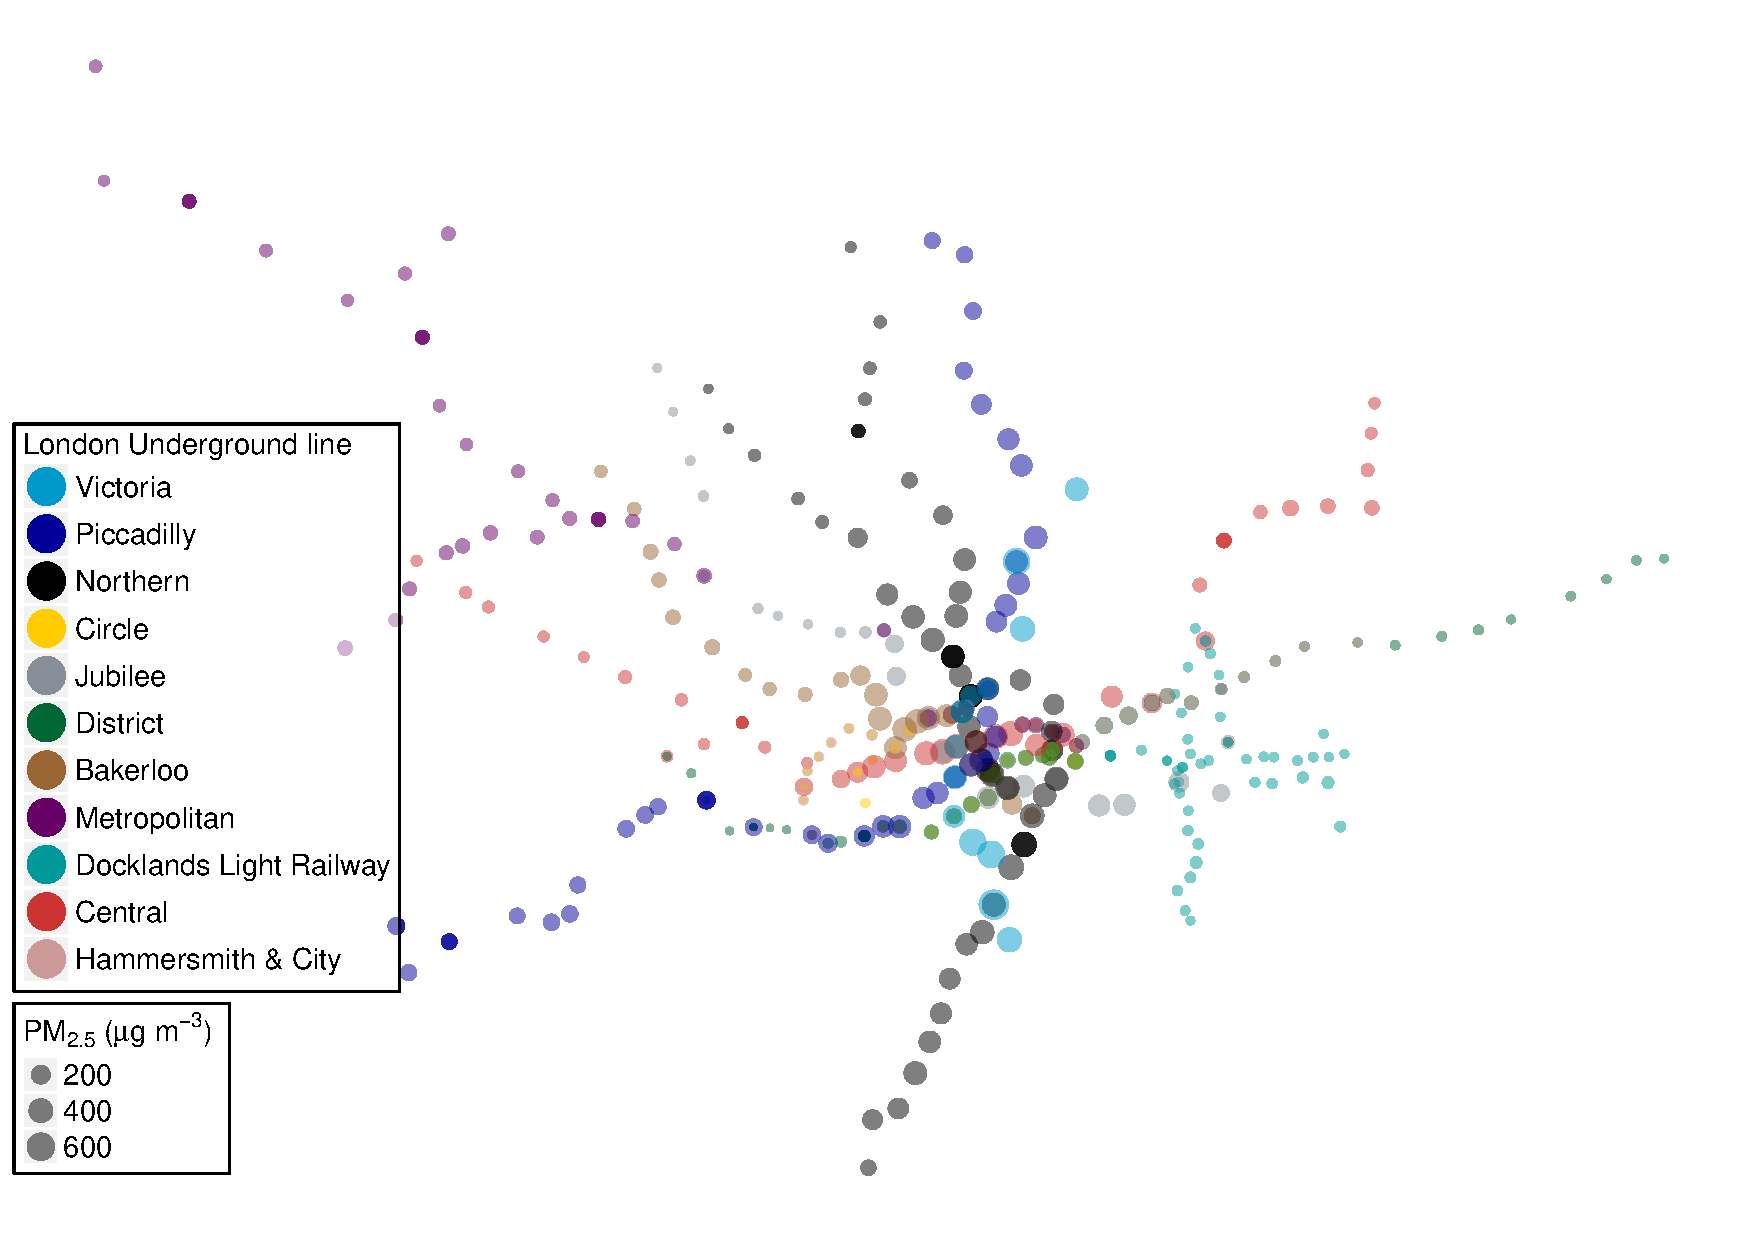
\includegraphics[scale=0.55]{tube_map_pm25}
\caption{Locations of tube stations and \gls{pm25} levels}
\label{fig:tube_map_pm25}
\end{figure}

As expected from the results of the previous sections, there looks to be a relationship between depth and \gls{pm25} concentrations, with stations in central London having higher concentrations, due to the lines being deeper and more frequently underground than in outer London. However as noted in \autoref{subsec:concentrations_v_depth} taking means at stations can hide variation, so whilst this figure is useful for giving a general impression of the spatial variation of concentrations, a more complicated approach might be more useful for modelling exposure.

%%%%%%%%%%%%%%%%%%%%%%%%%%%%%%
\subsection{PM build-up and dissipation}
\label{subsec:tube_air_build_up}
%%%%%%%%%%%%%%%%%%%%%%%%%%%%%%
In Figure \ref{fig:all_lines_individual_pm25_p1}, where timelines of \gls{pm25} are shown for each tube line, it is possible to see how on certain lines and at certain places concentrations fall to levels similar to background concentrations. To investigate how quickly the air in the carriage falls to these levels, from the elevated levels, the Jubilee line was taken as an example (due to it's clear differences between high and low concentrations). Figure \ref{fig:all_lines_individual_pm25_p1} has been re-created and annotated as Figure \ref{fig:decay_time_jubilee} below; a red line has been added to show the background \gls{pm25} concentration (taken from the 'Kensington and Chelsea - North Ken' background monitoring site), and black boxes and station names have been added to clarify the areas of interest.

\begin{figure}[H]
\centering
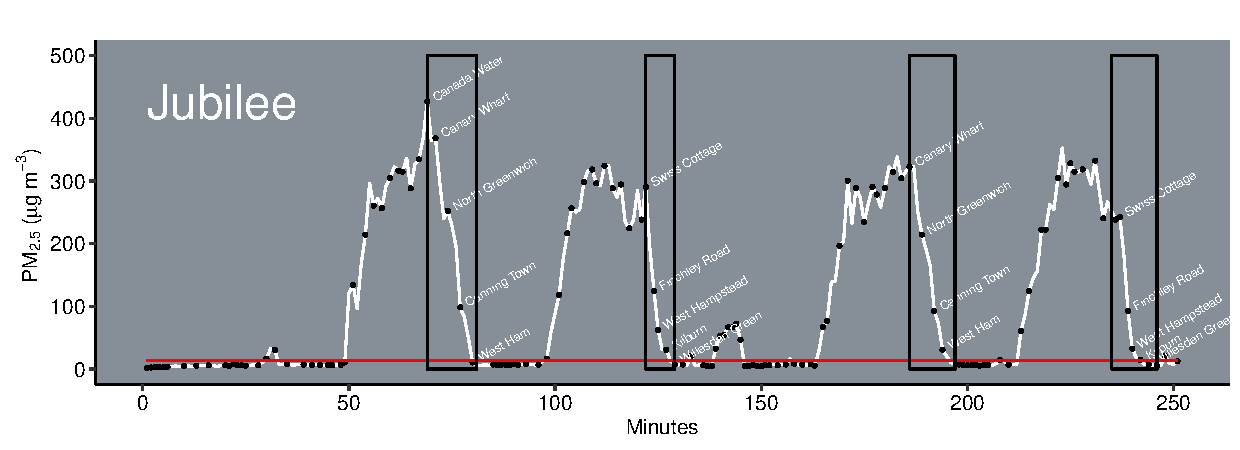
\includegraphics[scale=0.75]{decay_time_jubilee}
\caption{Locations of tube stations and \gls{pm25} levels}
\label{fig:decay_time_jubilee}
\end{figure}

Taking the first and third highlighted sections above, concentrations build-up inside the cabin while the train is underground, but then start to fall after Canada Water, reaching background levels by the time the train is at West Ham. The depth of these stations are, in order, Canada Water (18m), Canary Wharf (18m), North Greenwich (15m), Canning Town (2), and West Ham (0m). These stations do not have the step-by-step change in depth in the way that the concentrations do. If anything, the first three stations in this subset might be grouped as deep, and then the final two as surface. However the concentrations do not immediately change from high to background, they gradually decline. This suggests that in addition to depth being an indicator of concentrations inside the tube trains, distance from cleaner outside air, and it's exchange with air inside the cabin when the doors open, also effects concentrations. To elaborate, the concentrations between Canada Water and North Greenwich fall by about 40\%, despite there only being a small change in depth. I suggest that the change in concentrations is due to the doors opening at North Greenwich, and an air exchange happening with the air on the platform, which is cleaner 'platform air' than is the case at Canada Water, due to North Greenwich being closer to a surface station (Canning Town). 
Now taking the second and fourth sections highlighted in Figure \ref{fig:decay_time_jubilee} the stations under consideration are Swiss Cottage (17m), Finchley Road (3m), West Hampstead (5m), Kilburn (7m) and Willesden Green (5m). Here we see a similar pattern, in that the concentrations do not immediately drop to background levels in the way that might be expected if depth was the sole determinant. It takes a couple of stations (and subsequent doors opening and air exchange) for the air in the train cabin to be sufficiently replaced with cleaner outside air.

%%%%%%%%%%%%%%%%%%%%%%%%%%%%%%
\subsection{Train stock}
\label{subsec:tube_train_stock}
%%%%%%%%%%%%%%%%%%%%%%%%%%%%%%
Mean concentrations per line were now calculated (in the same manner as section \ref{subsec:line_averages}), but rather than grouping by line, the train stock data was linked, and boxplots created with that as the categorical variable (Figure \ref{fig:pm25_by_stock}) 

\begin{figure}[H]
\centering
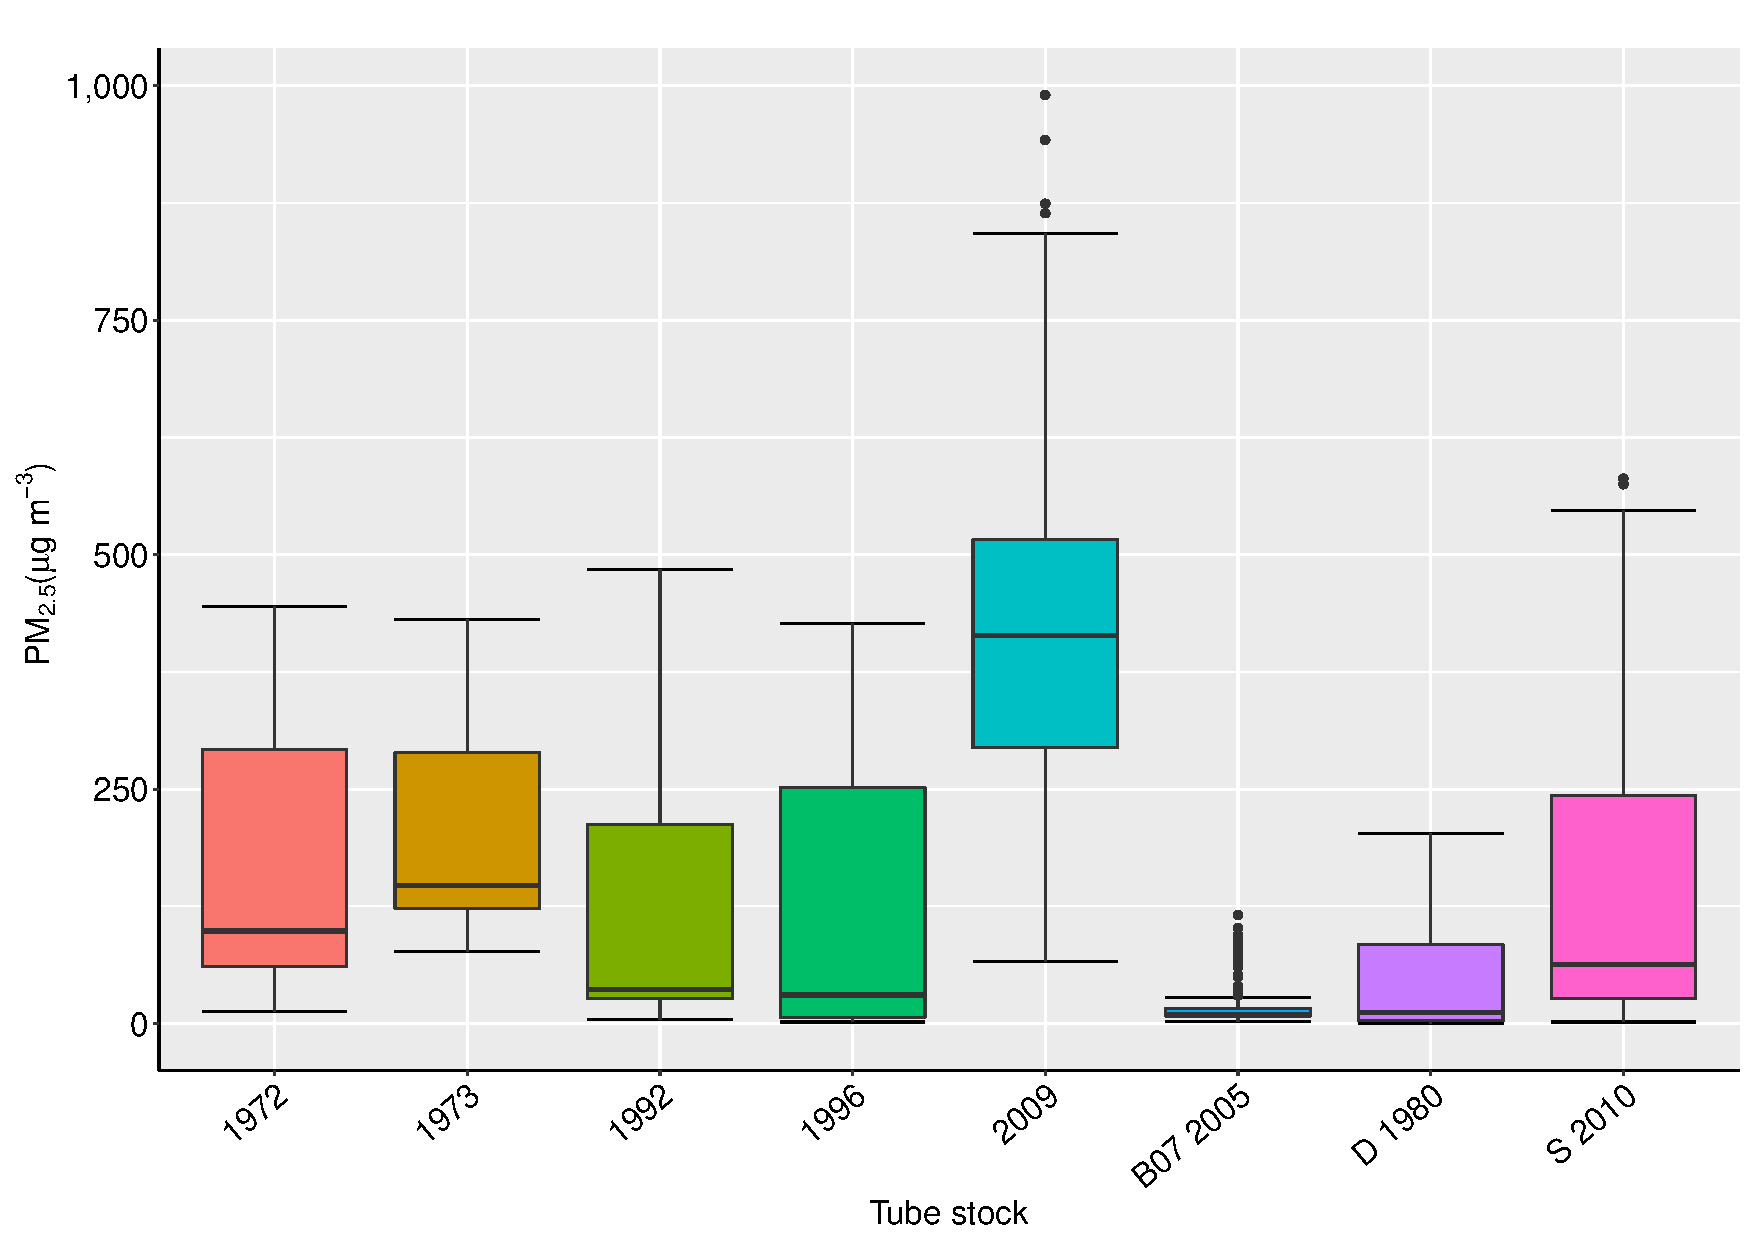
\includegraphics[scale=0.45]{pm25_by_stock}
\caption{\gls{pm25} $\mu \text{g m}^{-3}$ on the tube, summarised by stock type}
\label{fig:pm25_by_stock}
\end{figure}

There does not seem to be any clear pattern to \gls{pm25} concentrations when examining the data using train stock as a variable. Excluding the B07 2005 stock (as they are soley used on the DLR), the oldest trains (D 1980 stock) have the lowest concentrations, and the 2009 stock the highest. But they are only used on the District line and the Victoria lines respectively, and as we have seen there are large variations within the length of those lines which suggest that there are other factors (namely depth and distance from exposed station platforms) which are influential and not linked to train stock.

%%%%%%%%%%%%%%%%%%%%%%%%%%%%%%
\subsection{Revising LHEM exposure estimates}
\label{subset:revising_lhem_exposure}
%%%%%%%%%%%%%%%%%%%%%%%%%%%%%%
As discussed at the beginning of this chapter, whilst travelling on the London Underground network the \gls{ltdsx} subjects were assigned \gls{pm25} exposure concentrations of 95 $\mu \text{g m}^{-3}$ per minute. We can now see that this is a simplistic representation of the exposure found within the network. A final aim for this research area is to create a detailed spatial model layer which can be used for exposure assessments of the population of London while on the tube, however as an intermediary step, two \gls{ltds} subjects who used the London Underground during their day were chosen at random, and their exposure recalculated, but with mean line concentrations taken from this new data, to give an example of the possible effects using it will have. Their \gls{lhem} exposure (baseline in this instance) before this new method is shown in Figure \ref{fig:lhem_exposure_timeline}, with the exposure of 95 $\mu \text{g m}^{-3}$ while the subjects are on the tube, shown in blue.

\begin{figure}[H]
\centering
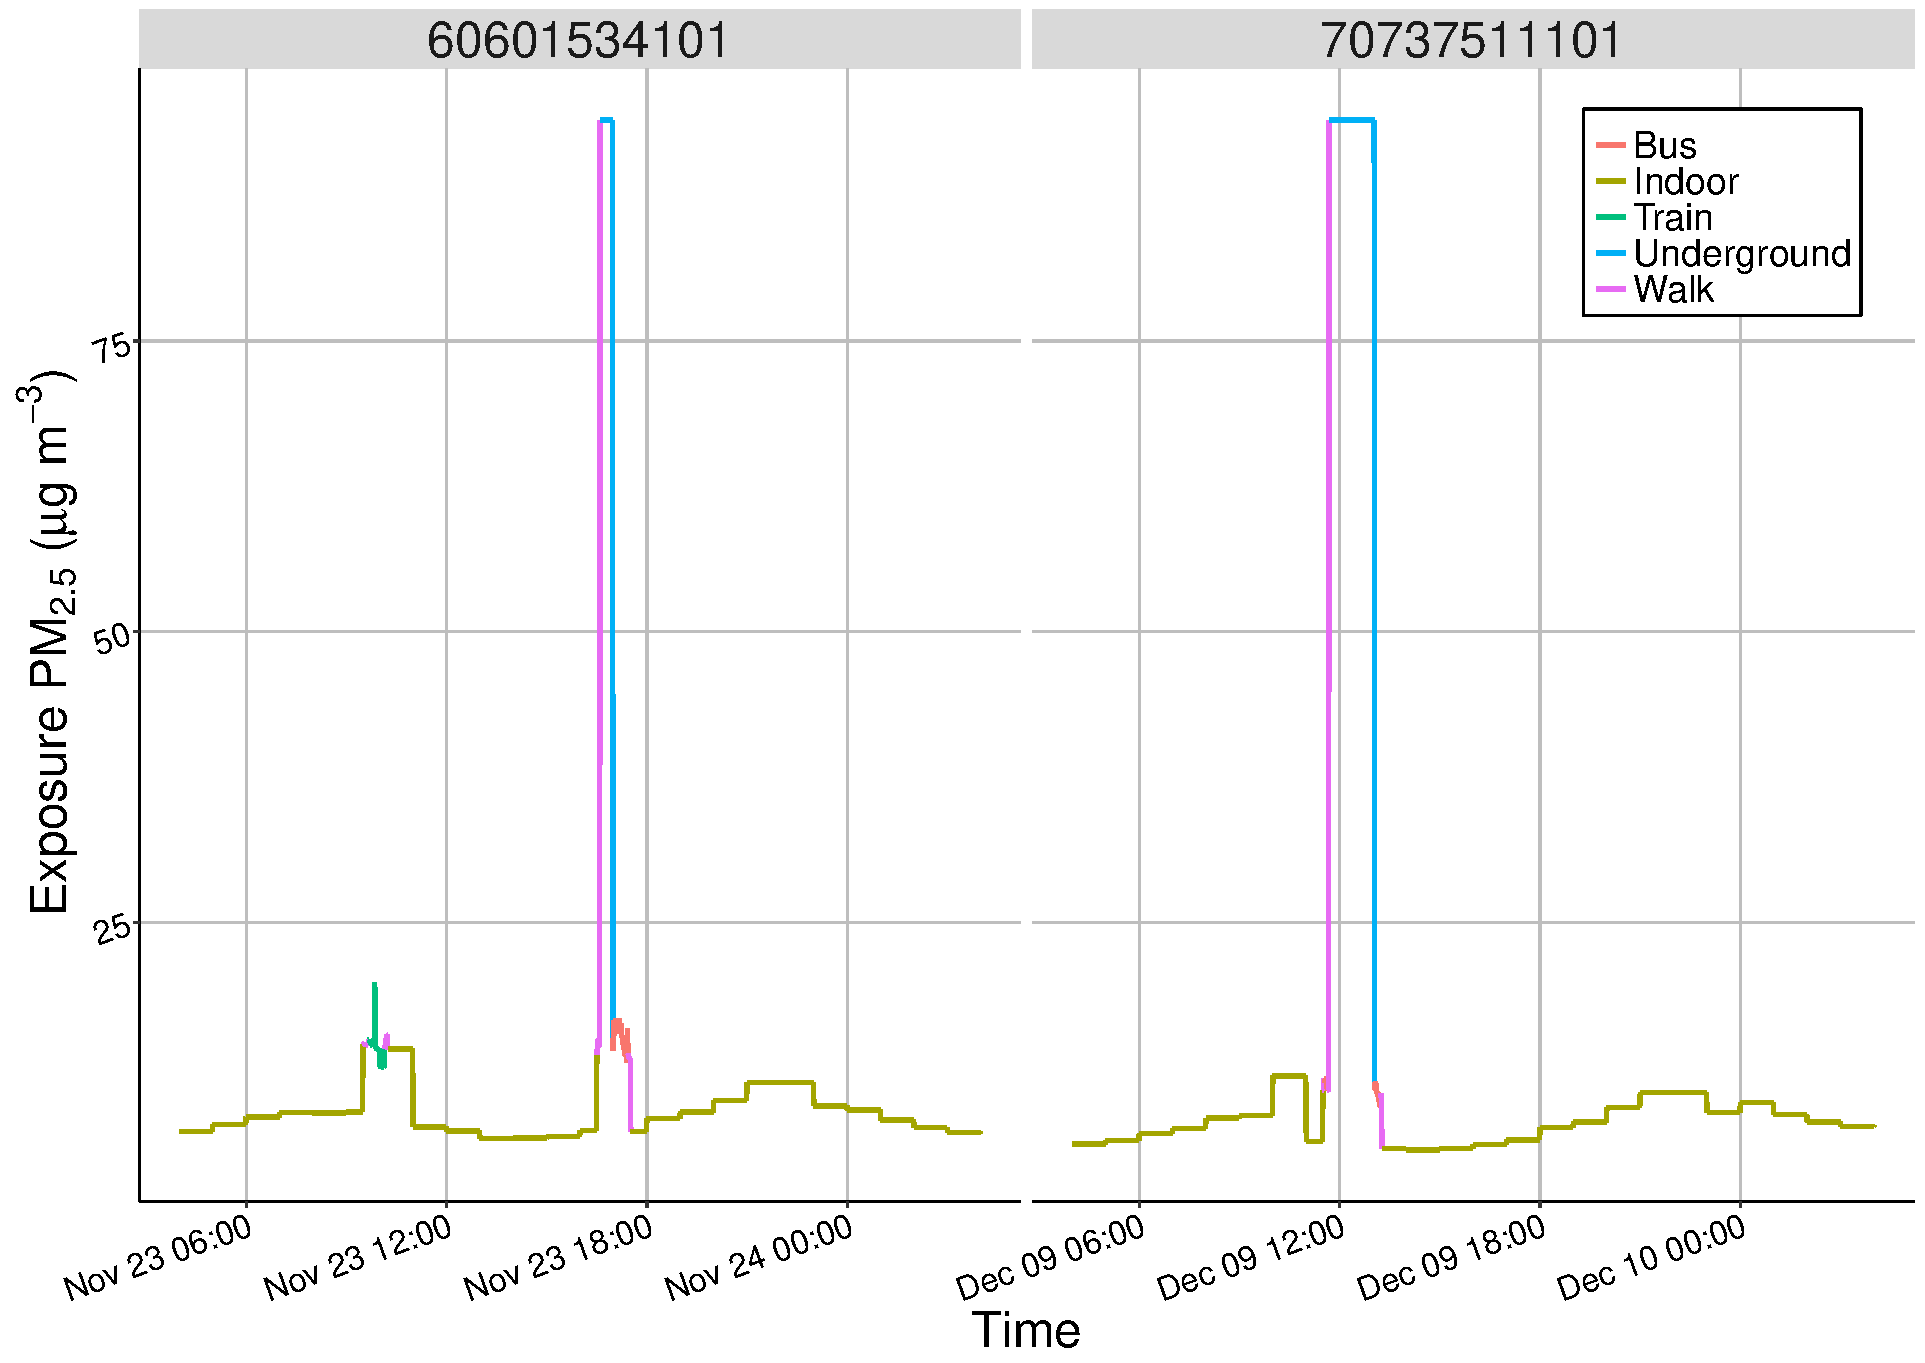
\includegraphics[scale=0.4]{recalculating_lhem_pre}
\caption{\gls{pm25} $\mu \text{g m}^{-3}$ exposure for \gls{lhem} subjects 60601534101 and 70737511101}
\label{fig:lhem_exposure_timeline}
\end{figure}

The mean daily exposure for these two subjects was 10.06 $\mu \text{g m}^{-3}$ and 12.69 $\mu \text{g m}^{-3}$ respectively. Subject 60601534101 begun their journey at Finsbury Park, and ended it at Arnos Grove, taking the Piccadilly line. The mean \gls{pm25} recorded on the Piccadilly line was 63 $\mu \text{g m}^{-3}$, and this is therefore substituted instead of the 95 $\mu \text{g m}^{-3}$ used. For subject 70737511101, they began their journey at Rayners Lane, and ended it Canning Town, taking the Metropolitan line for approximately the first third of their journey, and the Jubilee line for the remaining two thirds. So the first third of their journey the mean Metropolitan line concentration of 67 $\mu \text{g m}^{-3}$ is used, and for the second two thirds of their journey the mean Jubilee line concentration of 138 $\mu \text{g m}^{-3}$ is used. The new timelines are shown below in \autoref{fig:lhem_exposure_post_timeline}.

\begin{figure}[H]
\centering
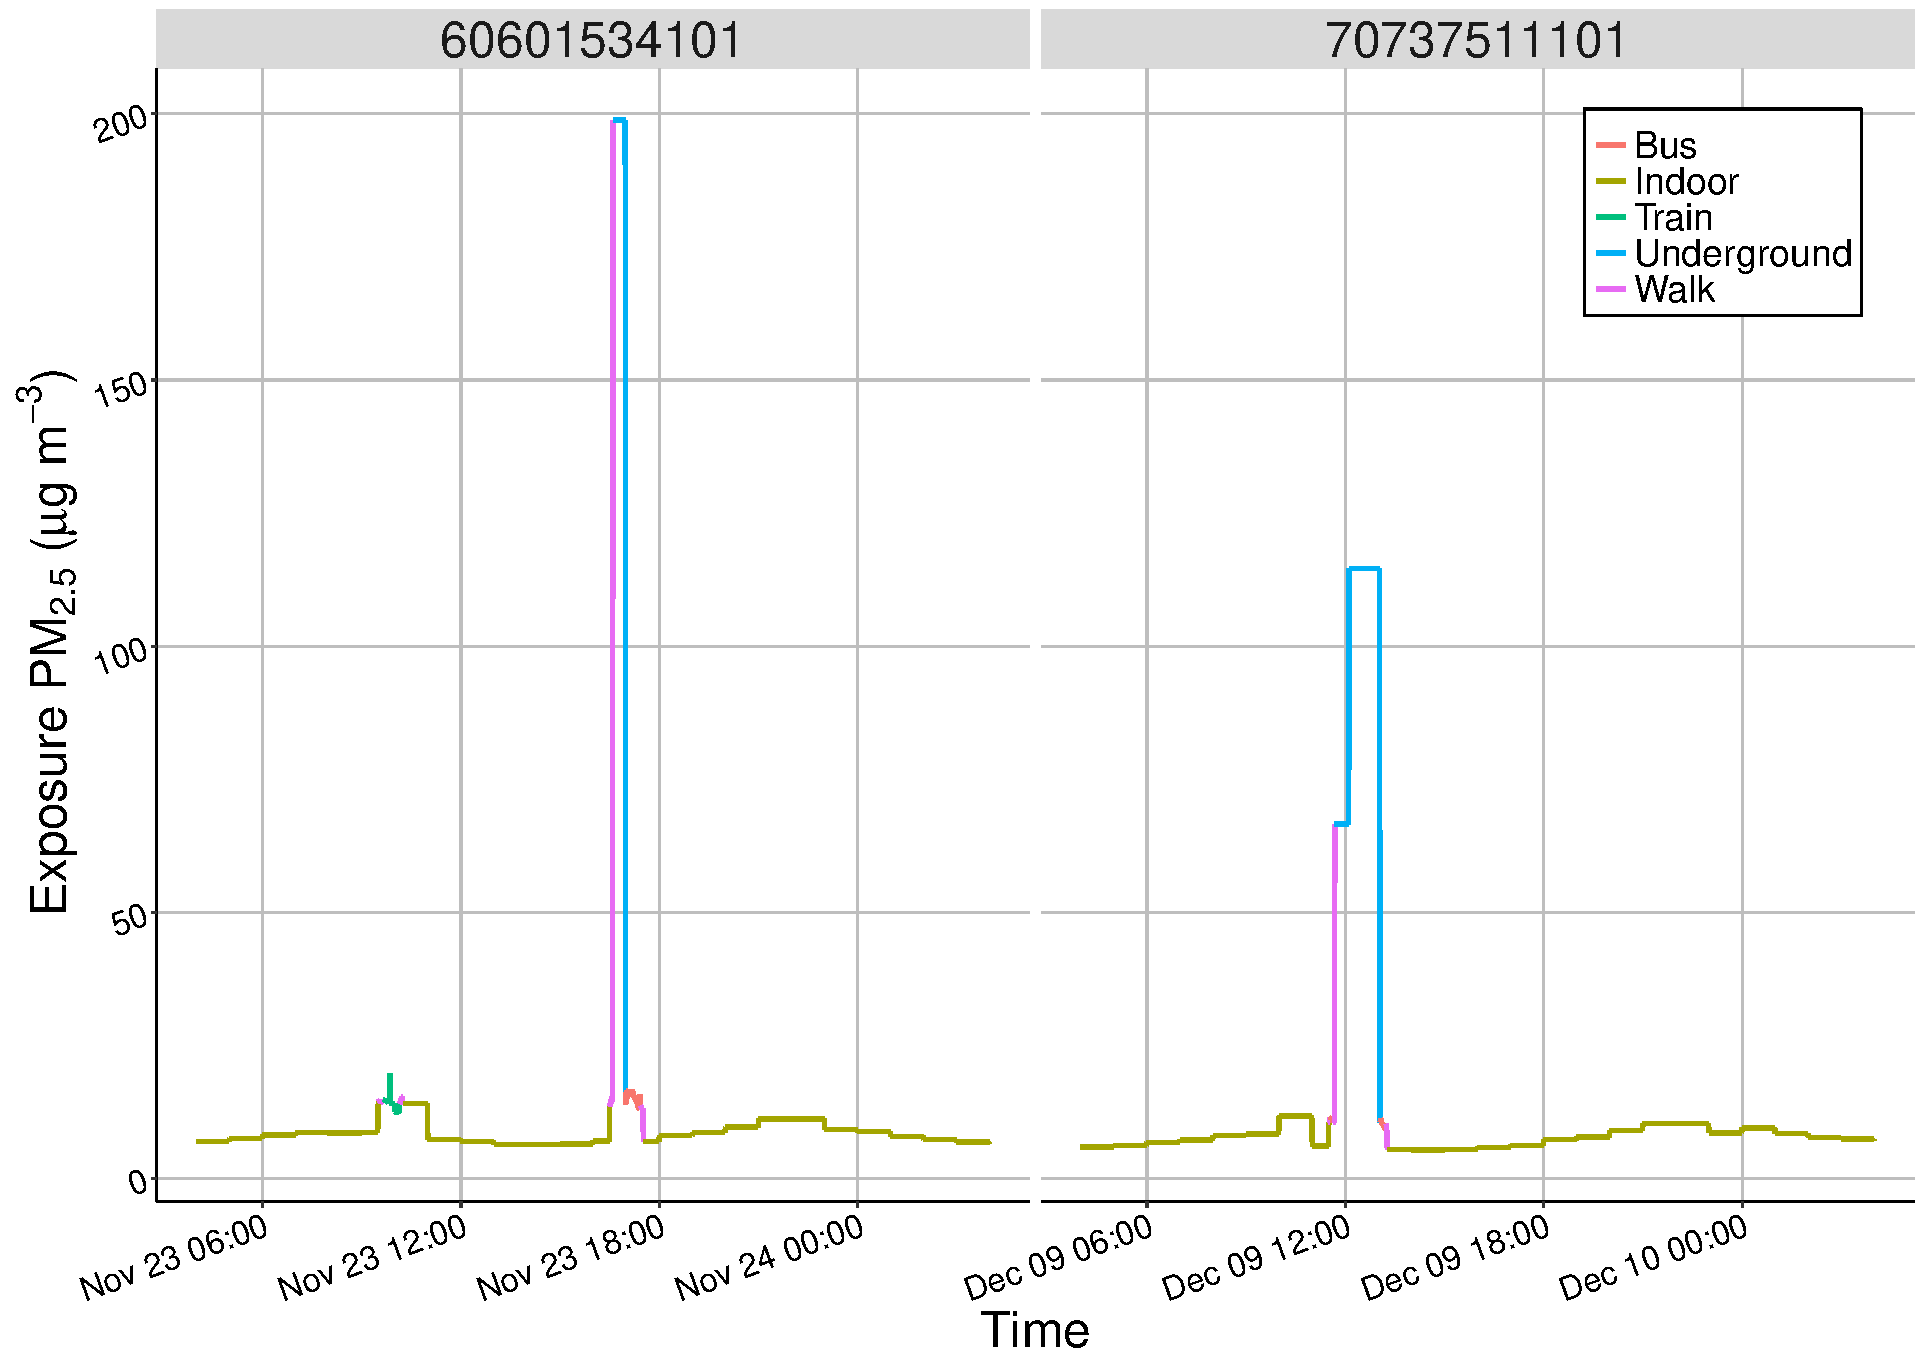
\includegraphics[scale=0.4]{recalculating_lhem_post}
\caption{Revised \gls{pm25} $\mu \text{g m}^{-3}$ exposure for \gls{lhem} subjects 60601534101 and 70737511101}
\label{fig:lhem_exposure_post_timeline}
\end{figure}

The new mean daily exposure for these two subjects, using the new London Underground data, was 11.73 $\mu \text{g m}^{-3}$ and 12.99 $\mu \text{g m}^{-3}$, an increase of 17\% and 2.4\% respectively. The former being higher, as although the journey was short the concentrations were much higher for that period than previously modelled. Alongside this increase in mean exposure, both subjects for a short period are also exposed to higher peaks in concentrations than in the old method.

%%%%%%%%%%%%%%%%%%%%%%%%%%%%%%
\section{Discussion}
\label{sec:3Discussion}
%%%%%%%%%%%%%%%%%%%%%%%%%%%%%%

%% What was good about this chapter
%% How does this study compare with other studies

This dataset is, to the best of my knowledge, the largest, most systematic, and detailed collection of \gls{pm25} concentrations on the London Underground. There are few studies which have studied \gls{pm25} on the tube, however in a review of exposure on metro systems  \cite{Nieuwenhuijsen2007} collated various studies, and specifically within London found ranges of between 130--200 $\mu \text{g m}^{-3}$, 157--247 $\mu \text{g m}^{-3}$, and 12--264 $\mu \text{g m}^{-3}$, mostly from the \cite{Adams2001a} studies which completed around sixty journeys on the tube in 2001. The data collected for this chapter is superior as the Adams work only collected data for short sections of repeat journeys on the Piccadilly, Bakerloo, Northern and District lines for comparison with other transport modes, and no spatial analysis was undertaken (or indeed possible as the data was collected on filters and therefore lacked spatial and temporal granularity). 

In addition to peer-reviewed academic work, the main other sources of \gls{pm25} measurements on the tube come from occupational health work commissioned by \gls{tfl}, the most well know being the "Assessment of health effects of long-term occupational exposure to tunnel dust in the London Underground" led by Hurley and published in 2003 (\cite{Hurley2003}). This was commissioned with the purpose of looking at occupational exposure to drivers and station staff, with only a small section concerning passengers, and therefore most of the results focus on the personal exposure of drivers and staff. There is no consideration of the variability by line, or within line, or an attempt at understanding the viability. In summary, the work completed and data collected is appropriate for for the purpose it was commissioned for, but not there are no spatial or temporal attributes linked to the data to enable further investigation or to use the results in other ways. Nonetheless the \gls{pm25} levels were found to be in the range 270--480 $\mu \text{g m}^{-3}$ on station platforms, and passengers average expose was taken as 200 $\mu \text{g m}^{-3}$, although a number of broad assumptions were made to arrive at this figure. As with \cite{Nieuwenhuijsen2007}, these concentrations are not dissimilar to those we measured.

By collecting \gls{pm25} concentrations and linking them to time-resolved location data across the whole of the network, and further calibrating the \gls{pm25} measurements using newly calculated scaling factors, we have been able to offer the most complete understanding of the variation and levels of pollutant in this environment that is used by millions of people everyday. There are however some issues and considerations with the methods and data collection that need discussion, and which might effect our findings. 

%% What are some of the issues and problems with the methods, and what makes the findings weak
Firstly, all of our measurements are taken from within the carriage of the tube. So whilst there is often discussion of stations within this chapter, this is actually the tube train (normally with doors open) pausing at the platform of a station for a minute or two before moving away again, and the reader must be careful not to misinterpret the findings as such. 

Another area that might warrant further refinement is around the effect that passenger numbers have on concentrations. The theory of the 'personal cloud', that being that a persons movements and activity can stir-up particles into the air that otherwise may have settled on surfaces. With so many people moving inside trains and on the platforms of the stations, this might contribute to increased concentrations independently of other factors i.e. the movement of the trains. This said, studies (\cite{Ferro2004a}) have found that this personal cloud effect to only increase concentrations by a few $\mu \text{g m}^{-3}$, which when set alongside the 100s of $\mu \text{g m}^{-3}$ being recorded are quite insignificant, and thus I feel that the effect of passenger numbers can be largely ignored in efforts to understand \gls{pm25} levels in this environment.

Similarly, \cite{Adams2001a} discusses that wind direction and outdoors concentrations may be linked to increased concentrations in the tube system, with particles being blown into the tunnels and recirculating. But with background concentrations of \gls{pm25} in London normally around the 10--15 $\mu \text{g m}^{-3}$ mark, it seems unlikely that pollutants from outside the system are contributing in a meaningful way to the high concentrations found (when the tube is in the underground environment anyway). 

Regarding the findings related to depth, these must also be considered alongside the fact that the depth data obtained and used in this research related to station platform depths, and was not detailed enough to enable understanding of depth between stations. This would have been useful particular for Section \ref{subsec:tube_air_build_up} (\nameref{subsec:tube_air_build_up}) where the build-up and dissipation of \gls{pm25} between stations was considered. Alongside monitoring equipment with a higher time resolution, say 3-4 seconds rather than 1 minute, it would be easier to understand how the concentrations vary between stations and along stretches of track.

A further complication to the findings we have so far, is that of ventilation settings and train stock. Some of the lines only have one stock-type running on them, but some lines have a variety. Also within these varieties different ventilation settings are available, and vary as to whether they are in use/functioning or not. It would be useful to repeat a sample of this data collected with a specific focus on ventilation to understand this variable more.

%% What use is this study
The data collected in this study is an important step forward in better estimating the exposure of people who live and commute in London (as was demonstrated with two random LHEM subjects). With further work, a dataset can be created which will allow vastly improved estimation of the exposure of millions of people travelling on the tube, which in most exposure studies involving London is not currently considered at all. Epidemiological studies are still geocoding peoples address or perhaps postcodes, and then taking annual concentration maps, normally with small ranges between the maximum and minimums, when there are millions of people every day who are spending prolonged periods of time in environments that have \gls{pm25} concentrations of over 500 $\mu \text{g m}^{-3}$. It might be that the there are strong links between people who use the London Underground for more than an hour a day, and those who develop chronic obstructive pulmonary disorder (\gls{copd}) issues. At the moment there has been no way to investigate this on a population level, but this research makes developing a research question about this subject now possible.

%% Should I look to say something here about susceptible groups?

%% What might be done next to continue this work
Future work in this area should focus on creation of a geographically defined data layer or database which can be used alongside passenger modelling (such as done by a Dr Reades, a colleague in the Geography department of \gls{kcl} (\url{https://www.youtube.com/watch?v=F6qsh1KBW-E}).

\begin{figure}[H]
\centering
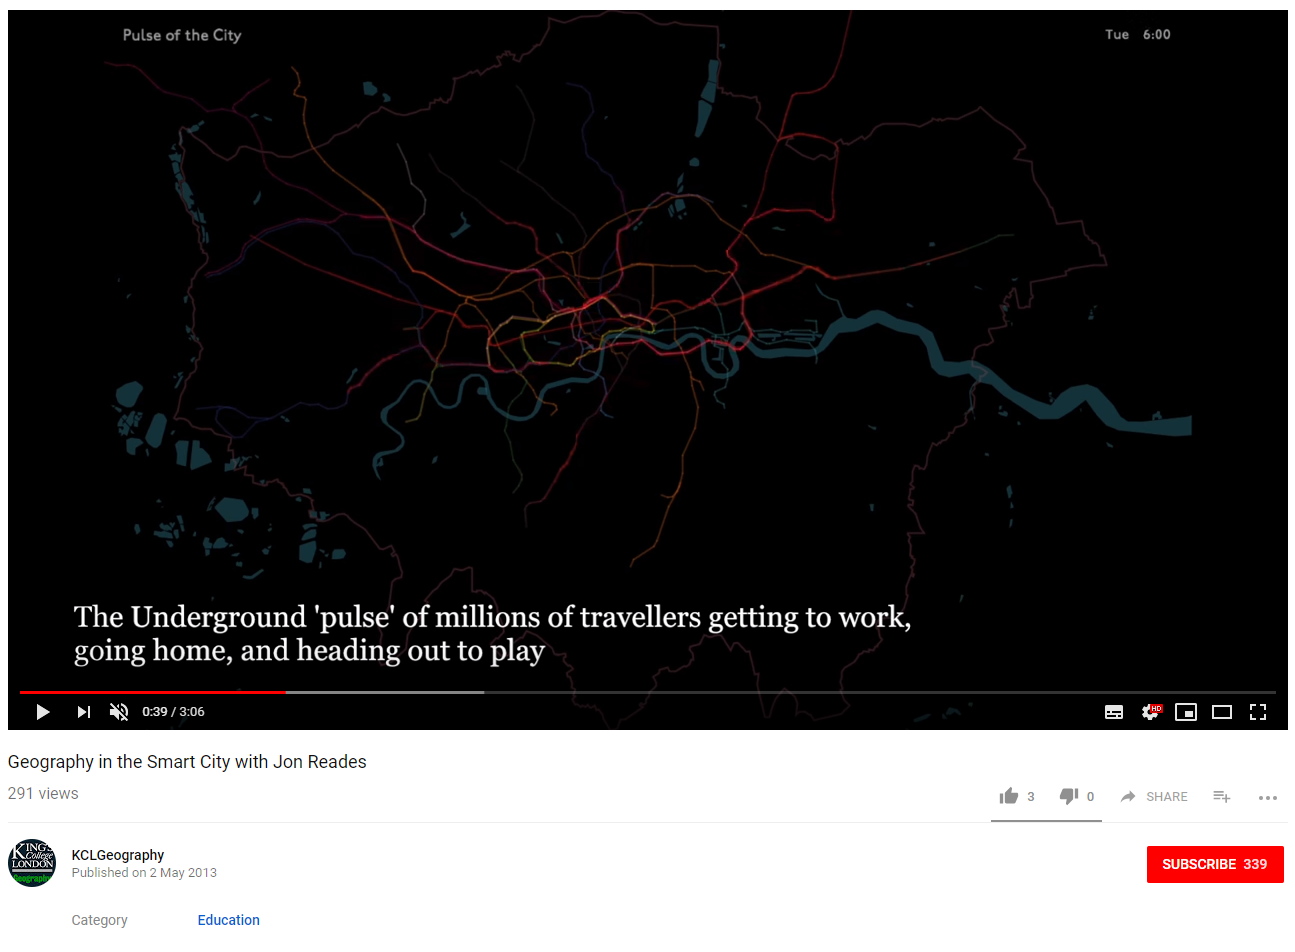
\includegraphics[scale=0.4]{images/pulse_of_london.png}
\caption{Dr Reades explaining the 'pulse of London' through geographical data}
\label{fig:pulse_of_london}
\end{figure}

This dataset should be sufficiently geographically defined, to have different exposure estimates related to each section of each tube line, rather than the intermediate step used in Section \ref{subset:revising_lhem_exposure} whereby line means were calculated. Preferably it should also take into account the direction of travel, as this was seen to alter \gls{pm25} exposure dramatically. One option would be to create a Tube network within a pgRouting database, and assign the concentrations as 'cost parameters' to each stretch of the network. Once built this would allow input of an origin and destination, and then the algorithms would calculate a route between the two stations that minimised exposure, with an output of exposure along the route. Although the LHEM currently makes use of the TfL routing API for this step of the model, and therefore a layer that can be easily incorporated to this step would be a more appropriate approach. Each minute that an individual is on the Tube would be a location and timestamp, and also a field containing the name of the Tube line the journey is on, so these coordinates could be 'snapped' to the nearest Tube segment, for the appropriate line of travel, and then the relevant concentrations extracted from the line data and assigned to that minute of travel.

%%%%%%%%%%%%%%%%%%%%%%%%%%%%%%
\section{Conclusions}
\label{sec:3conclusions}
%%%%%%%%%%%%%%%%%%%%%%%%%%%%%%

\gls{pm25} data collected on the London Underground varies between 0 $\mu \text{g m}^{-3}$ and 990 $\mu \text{g m}^{-3}$, with a mean of 129 $\mu \text{g m}^{-3}$ and a median of 63 $\mu \text{g m}^{-3}$.

%%%%%%%%%%%%%%%%%%%%%%%%
%%%%%% \subsection{Timeline concentrations}

There is a large variation when comparing lines against each other, and between sections of the same line. For example the Victoria line has concentrations of 990 $\mu \text{g m}^{-3}$ in some places, but a mean of 436 $\mu \text{g m}^{-3}$ and a minimum of 66 $\mu \text{g m}^{-3}$.

%%%%%%%%%%%%%%%%%%%%%%%%
%%%%%% \subsection{Line averages}

When ranked in decreasing order of mean \gls{pm25} concentrations, the results are; Victoria Line (436 $\mu \text{g m}^{-3}$), Northern (219 $\mu \text{g m}^{-3}$), Piccadilly (199 $\mu \text{g m}^{-3}$), Bakerloo (164 $\mu \text{g m}^{-3}$), Central (119 $\mu \text{g m}^{-3}$), Jubilee (115 $\mu \text{g m}^{-3}$), Metropolitan (67 $\mu \text{g m}^{-3}$), Circle (41 $\mu \text{g m}^{-3}$), District (40 $\mu \text{g m}^{-3}$), Hammersmith \& City (36 $\mu \text{g m}^{-3}$), Docklands Light Railway (18 $\mu \text{g m}^{-3}$) . Stations and sections of lines also have large variation. The Southern section of the Victoria line had some of the highest concentrations, particularly on the stretch of track between Brixton, Stockwell and Victoria with concentrations of 400-500 $\mu \text{g m}^{-3}$, compared to many stretches of track on more exposed lines such as the Circle, Hammersmith \& City and the Metropolitan lines where concentrations are often  less than 10 $\mu \text{g m}^{-3}$

%%%%%%%%%%%%%%%%%%%%%%%%
%%%%%% \subsection{Concentrations v. Depth}

Increasing depth was considered to be an indicator of increasing \gls{pm25} concentrations, illustrated by the linear relationships seen in Figure \ref{fig:concentrations_depth_summary} which looked at average concentrations by line and plotted them against average depth. However when this plot was dis-aggregated and considered by individual line, station, and direction of travel, this relationship became more complex. There were high concentrations recorded while on the tube at stations that are not particularly deep, and conversely low concentrations recorded while on the tube at stations that are very deep. The explanation for this variation is due to the environments immediately previously experienced by the train, and distance from those environments. Trains that have just exited areas of high concentrations bring polluted air with them which takes time to dissipate, and conversely tube trains that have been in cleaner air take a little while for concentrations in the carriages to increase. This increase and decrease seems likely to mainly happen at platforms when doors are opened and closed, but also to a lesser degree during movement of the train (both of which need further investigation).

%%%%%%%%%%%%%%%%%%%%%%%%
%%%%%% \subsection{Spatial distribution of tube air quality}

The spatial representation of the stations in London, ignorant of direction of travel and depth data, showed that higher concentrations tend to be found in central London areas.

%%%%%%%%%%%%%%%%%%%%%%%%
%%%%%% \subsection{Revising LHEM exposure estimates}

Finally, by calculating simplistic line averages in lieu of a more complex dataset that will be created in the future, two randomly chosen \gls{lhem} daily exposure estimates were re-calculated. Both subjects daily exposure increased, one by 17\% and one by 2\%. Repeating this new method across the entire tube-using population of London is likely to lead to a general increase in exposure from the \gls{lhem}, but with some people experiencing lower overall exposure (due to only travelling on section of the tube that are cleaner than previously presumed).